\documentclass{article}
\usepackage[utf8]{inputenc}
\usepackage[margin=1in]{geometry}
\usepackage[colorlinks]{hyperref}
\usepackage{graphicx}
\usepackage{caption}
\usepackage{color}
\usepackage{subcaption}
\usepackage{float}
\makeatletter
\renewcommand\paragraph{\@startsection{paragraph}{4}{\z@}%
            {-2.5ex\@plus -1ex \@minus -.25ex}%
            {1.25ex \@plus .25ex}%
            {\normalfont\normalsize\bfseries}}
\makeatother
\setcounter{secnumdepth}{4} % how many sectioning levels to assign numbers to
\setcounter{tocdepth}{4}    % how many sectioning levels to show in ToC
\begin{document}
\title{\textbf{CS6011: Kernel Methods for Pattern Analysis}
\\
\textbf{Programming Assignment 1}
}
\author{Aravind Sankar CS11B033 \\
Ramnandan SK CS11B061 \\
Adit Krishnan CS11B063 \\[0.2in]
Group 2
}
\floatplacement{figure}{H}
\maketitle
\tableofcontents 
\newpage
\section{Objective of the assignment}
The basic goal of this assignment is to use linear models of regression to do 2 Function Approximation tasks, namely Polynomial Curve fitting on Dataset 1 (univariate) and Surface Fitting using Gaussian Basis functions for Dataset 2 (bivariate). Here, the means of the Gaussians used are the centers of clusters obtained using K-means clustering of the training data. The experimental results obtained are to be summarized using plots obtained on varying different model parameters.
\section{Dataset 1}

\subsection{Generation}
The given function to be approximated is shown below :

\[ f(x) = e^{\cos(2 \pi x)} \]
\[ x \in (0,1) \]

\begin{flushleft}
To generate points from this function, we randomly generated points $x \in (0,1)$ and found the function value $f(x)$ at each point, and added to it Gaussian Noise with mean $\mu = 0$ and standard deviation $\sigma = 0.1$. 3 different training sets were generated, of sizes 20, 100 and 1000. The size of the validation and test set generated were 50 each.
\end{flushleft}

\subsection{Model creation}
\begin{flushleft}
As the goal is to fit a polynomial function to the given data, we need to decide on the degree $M$ of the polynomial which decides the model complexity. 

Through the plots, we show the variation of model outputs and RMS errors on varying different 
parameters and our analysis of the results to choose the best model.

\end{flushleft}
\newpage
\subsection{Results}

\subsubsection{Plots of approximated functions - Question 1}
%\paragraph{Effect of varying $M$}
The following plots showing variation of the polynomial w.r.t degree of polynomial $M$, for training dataset of size $N = 20$. Each plot shows the data points \textcolor{green}{x}, the target function \textcolor{blue}{$f(x)$}  and the approximated polynomial \textcolor{red}{$y(x,\bar{w})$} 
\begin{figure}[H]

\begin{subfigure}{.5\textwidth}
\centering
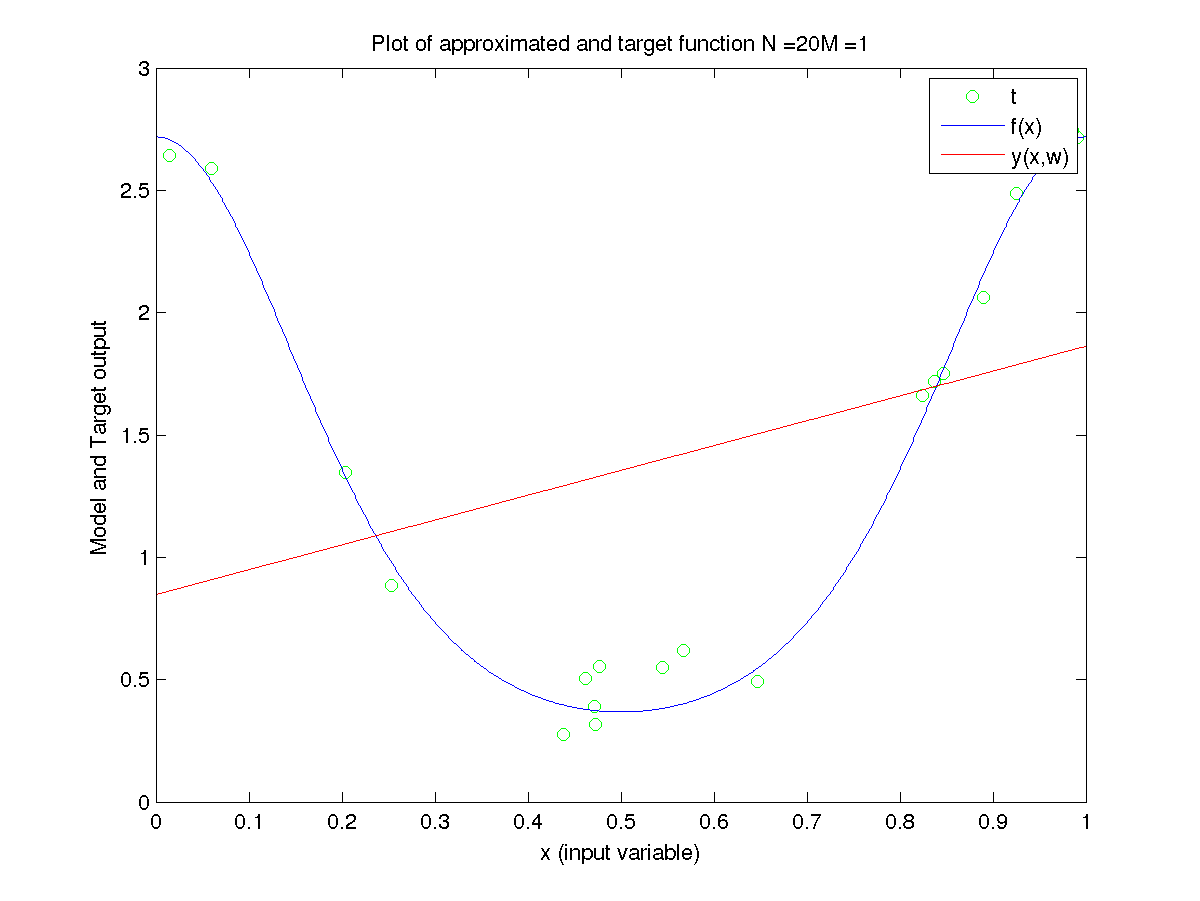
\includegraphics[width=\linewidth]{VaryingM_N20M1}
\caption{N = 20 M = 1}
\end{subfigure}
\begin{subfigure}{.5\textwidth}
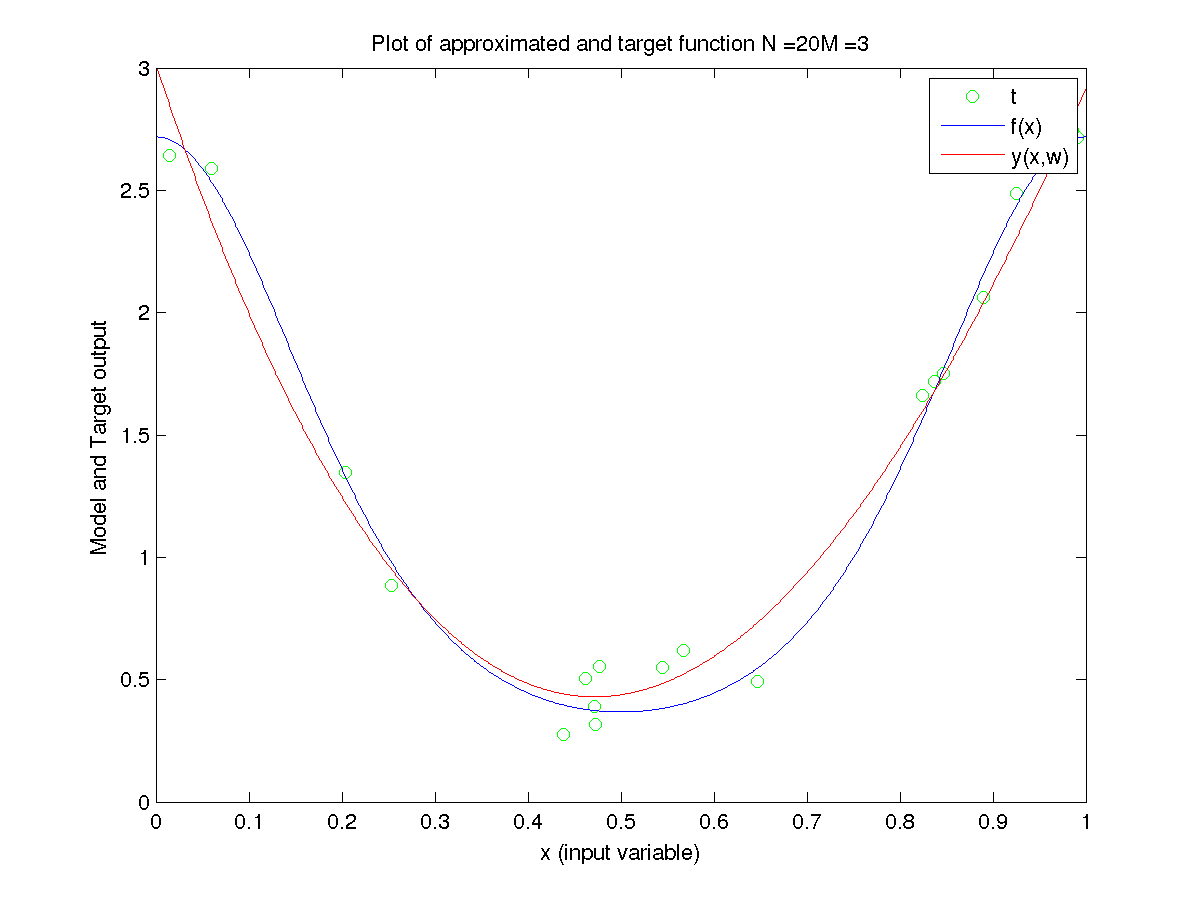
\includegraphics[width=\linewidth]{VaryingM_N20M3}
\caption{N = 20 M = 3}
\end{subfigure}


\begin{subfigure}{.5\textwidth}
\centering
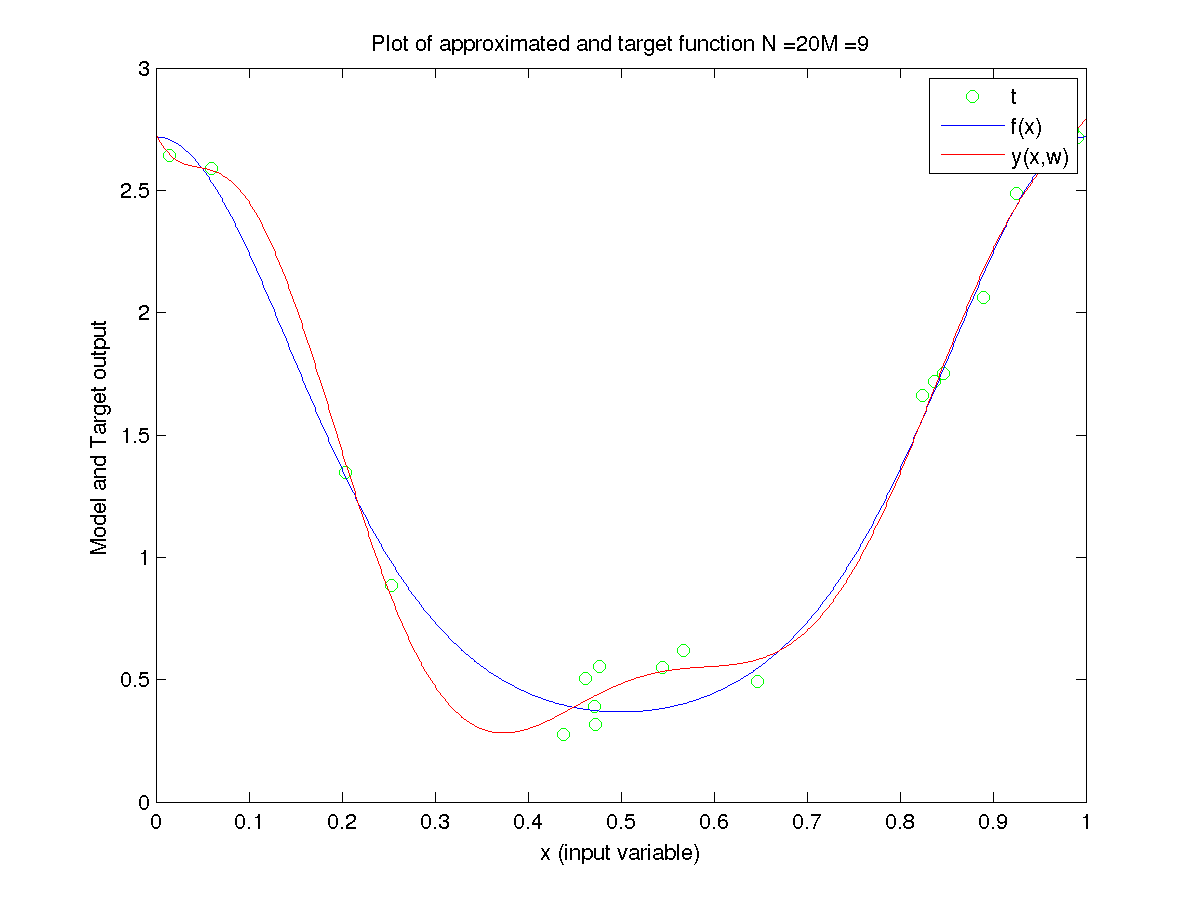
\includegraphics[width=\linewidth]{VaryingM_N20M9}
\caption{N = 20 M = 9}
\end{subfigure}
\begin{subfigure}{.5\textwidth}
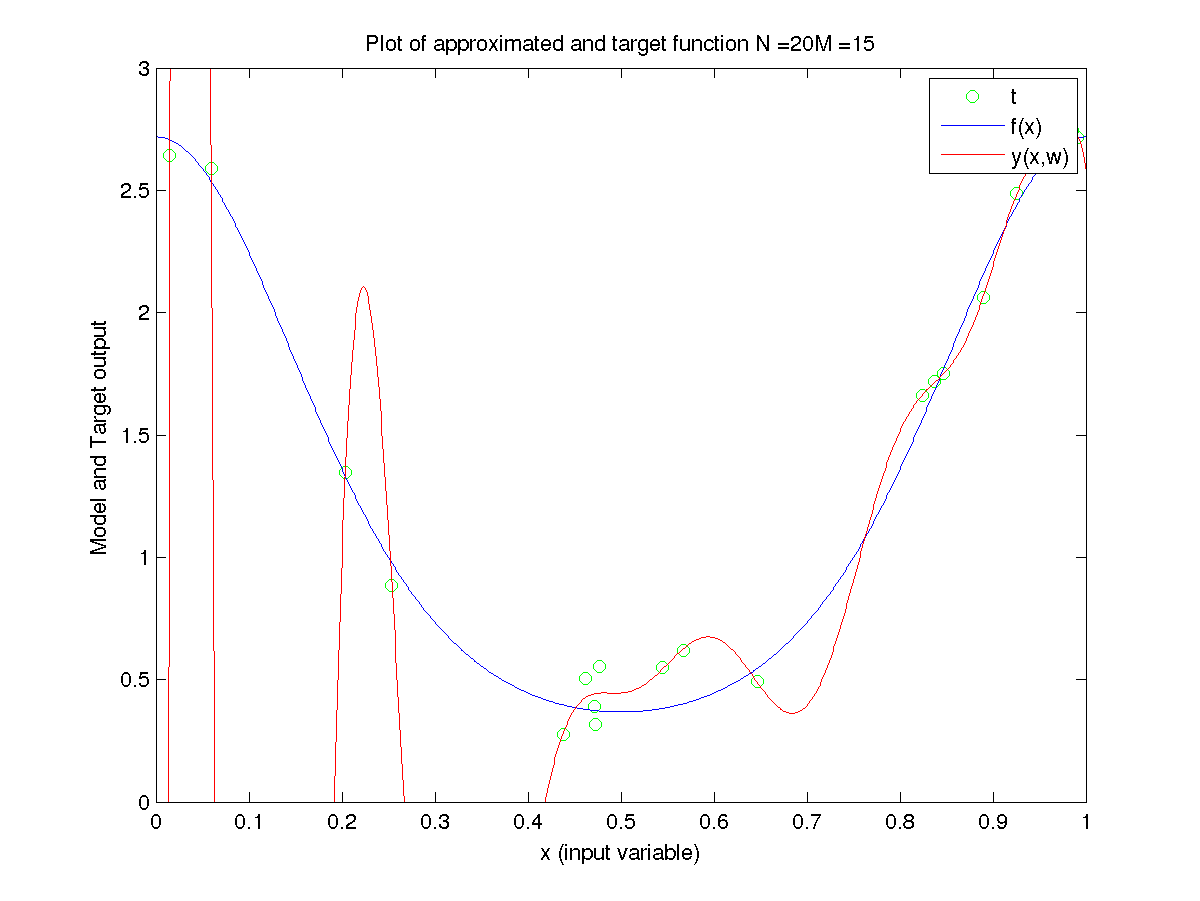
\includegraphics[width=\linewidth]{VaryingM_N20M15}
\caption{N = 20 M = 15}
\end{subfigure}



\end{figure}
\textbf{Observations :}

\begin{itemize}
\item We chose the training dataset with 20 points to clearly show the overfitting problem (for large model complexities) in the absence of regularization. 
\item Notice that the model with complexity 3 is very close to the true function.
\item For complexities 9 and 15, due to the small number of training data points, we observe overfitting which leads to significant deviation from the underlying target function.

\end{itemize}
\newpage

%\paragraph{Effect of varying $N$}
\begin{flushleft}
The following plots show the different polynomials obtained on varying the training dataset size $N$. Each of these plots are shown for 2 values of $M$, 9 and 15.
The plots for N = 20 and these values of M has already been plotted above. So, the following plots correspond to training dataset sizes of 100 and 1000. 
\end{flushleft}
\begin{figure}[H]

\begin{subfigure}{.5\textwidth}
\centering
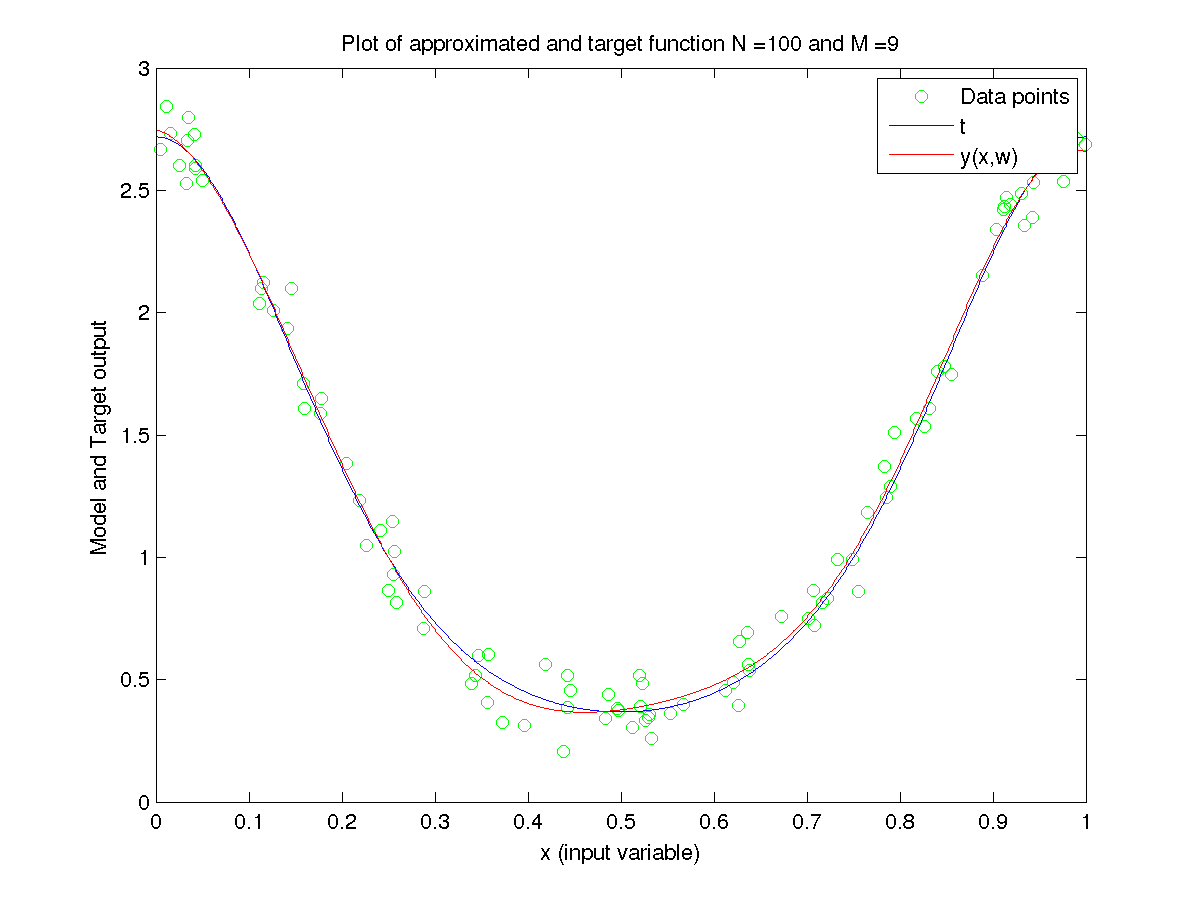
\includegraphics[width=\linewidth]{VaryingN_N100M9}
\caption{N = 100 M = 9}
\end{subfigure}
\begin{subfigure}{.5\textwidth}
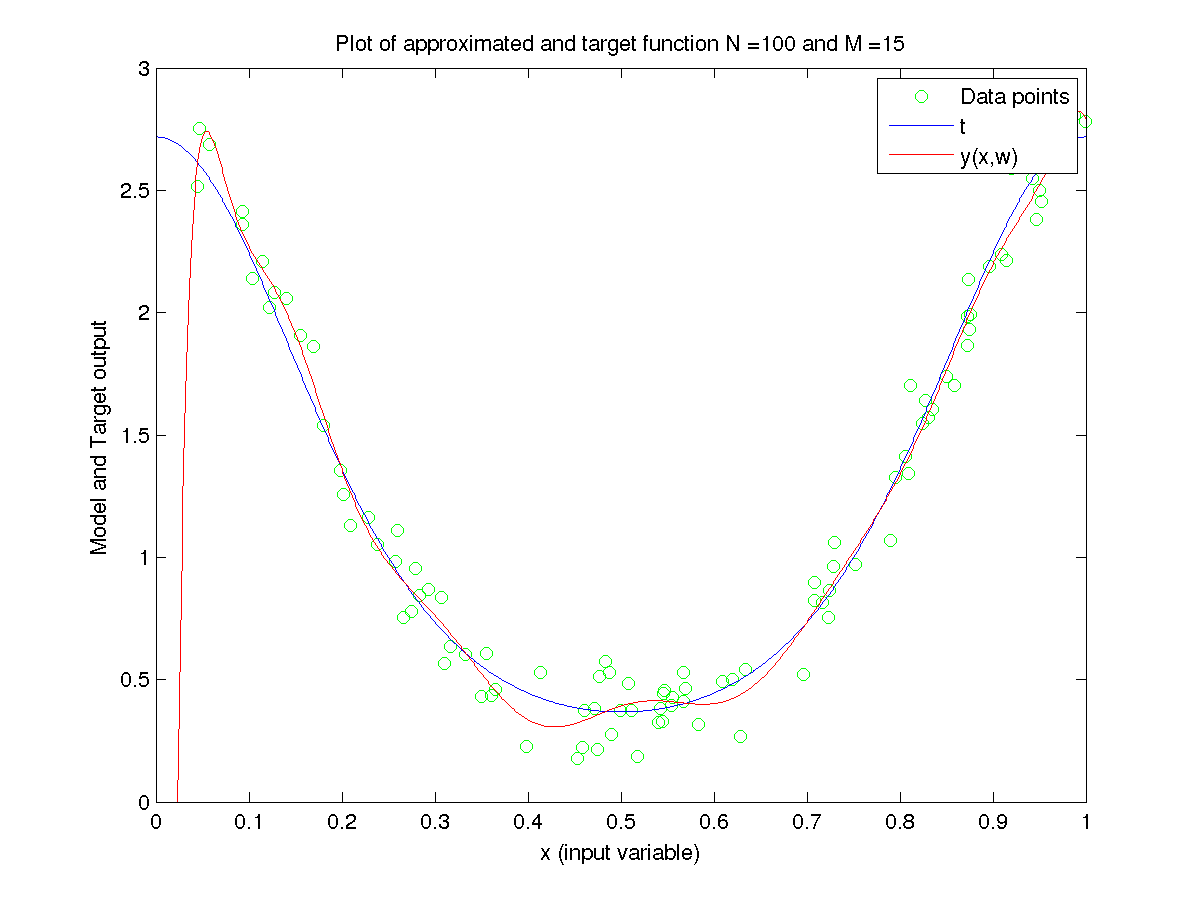
\includegraphics[width=\linewidth]{VaryingN_N100M15}
\caption{N = 100 M = 15}
\end{subfigure}


\begin{subfigure}{.5\textwidth}
\centering
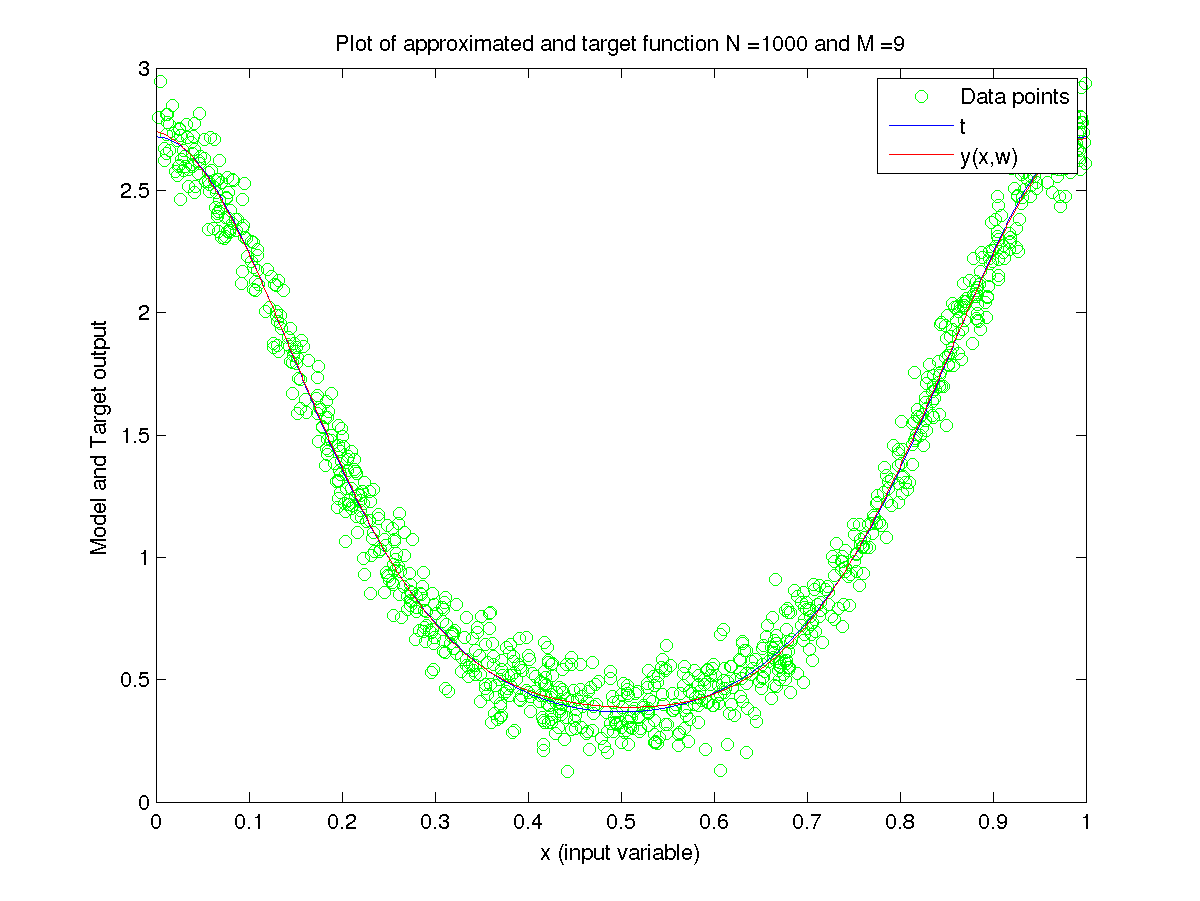
\includegraphics[width=\linewidth]{VaryingN_N1000M9}
\caption{N = 1000 M = 9}
\end{subfigure}
\begin{subfigure}{.5\textwidth}
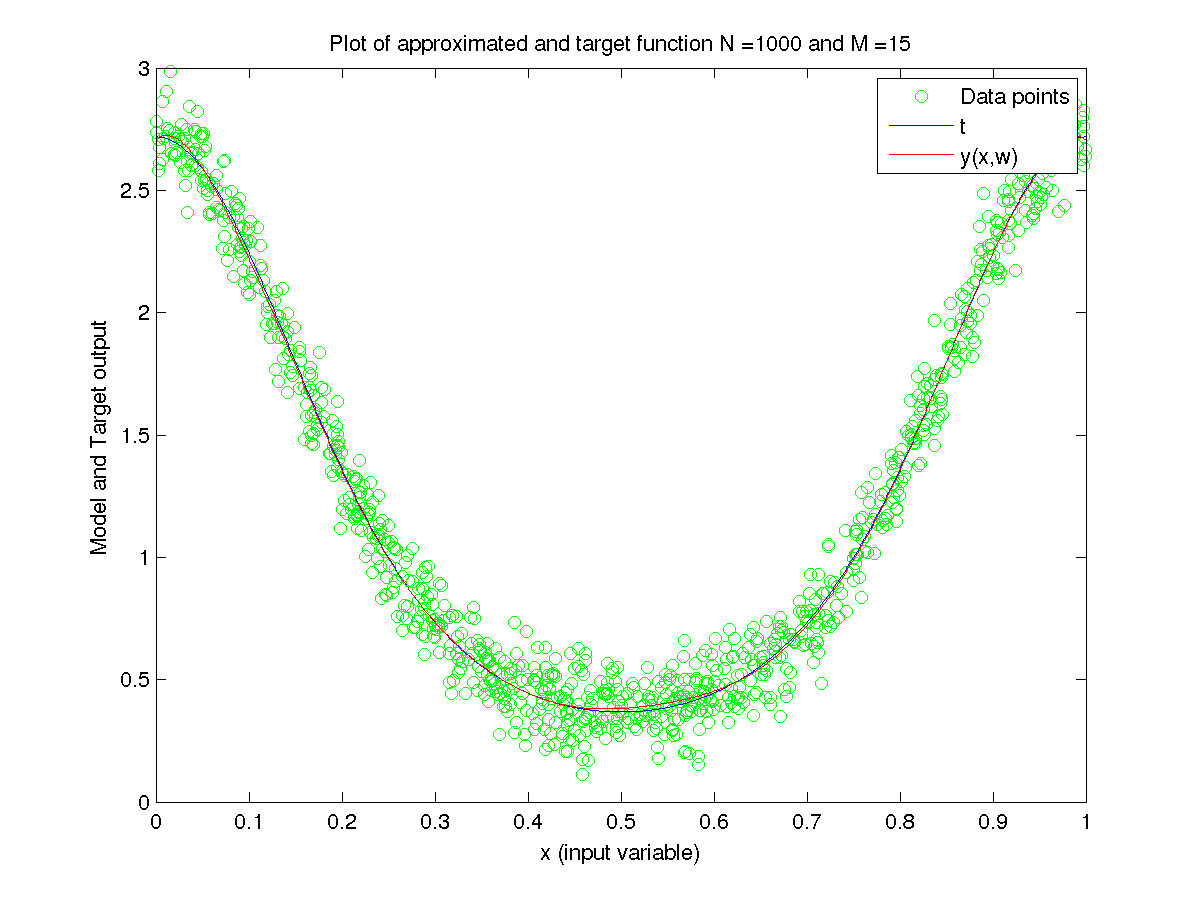
\includegraphics[width=\linewidth]{VaryingN_N1000M15}
\caption{N = 1000 M = 15}
\end{subfigure}



\end{figure}

\textbf{Observations: }
\begin{itemize}
\item We observe that Model complexity $M=9$ almost matches the target function for both datasets since there are sufficient samples.
\item However, Model complexity $M=15$ leads to slight overfitting and hence some deviation from $f(x)$ in case of $N = 100$.
\item However, for the 1000 sample dataset($N = 1000$) both models are almost overlapping with the target function due to the sufficiency of training points.
\item Next we look at the effect of regularization.
\end{itemize}
\newpage

%\paragraph{Effect of varying regularization parameter $\lambda$}
\begin{flushleft}
The following plots show the effects of varying the regularization parameter $\lambda$ on the curve fit. Since the overfitting effect is pronounced only for a small training set, these plots correspond to the 20 point training set and model complexity $M = 9$.
\end{flushleft}
\begin{figure}[H]

\begin{subfigure}{.5\textwidth}
\centering
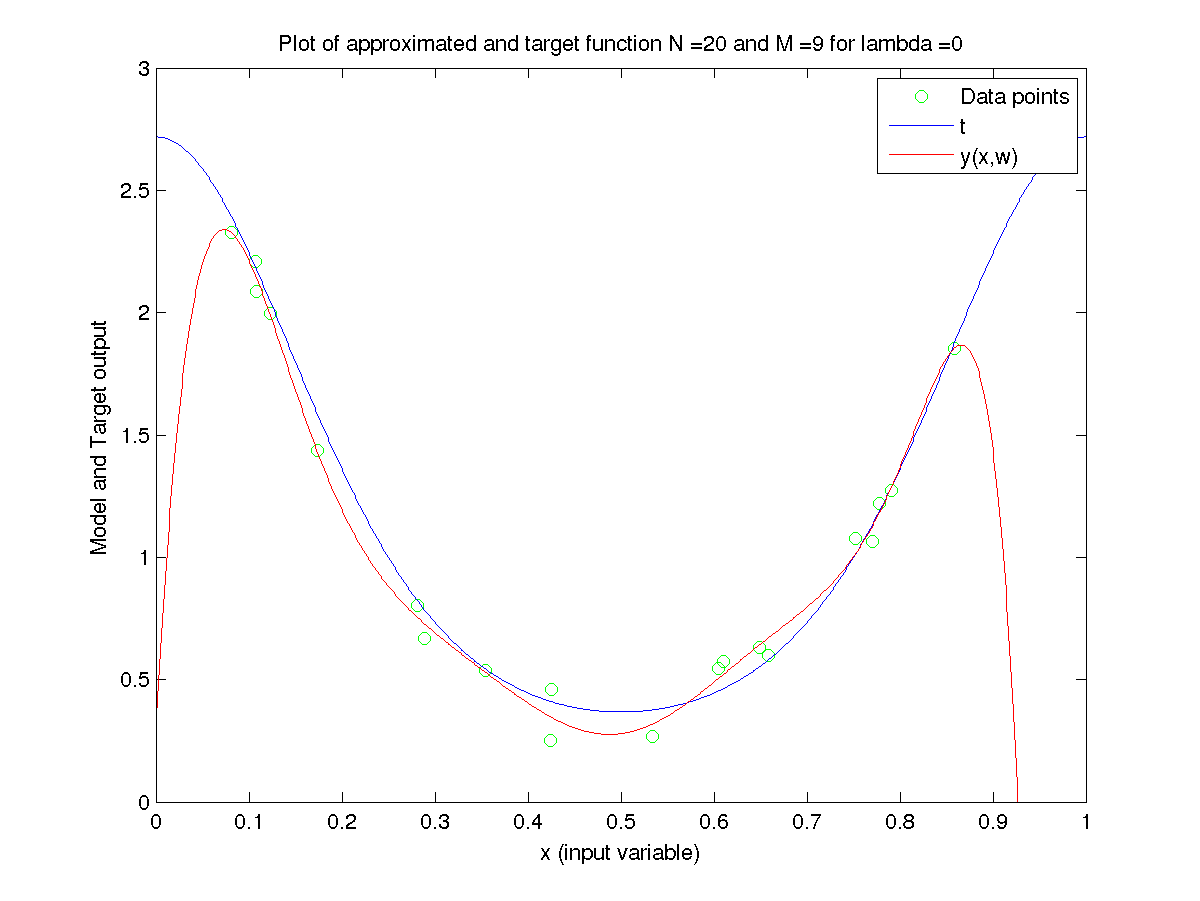
\includegraphics[width=\linewidth]{Varyinglambda_N20M9lambda0}
\caption{$\lambda$ = 0}
\end{subfigure}
\begin{subfigure}{.5\textwidth}
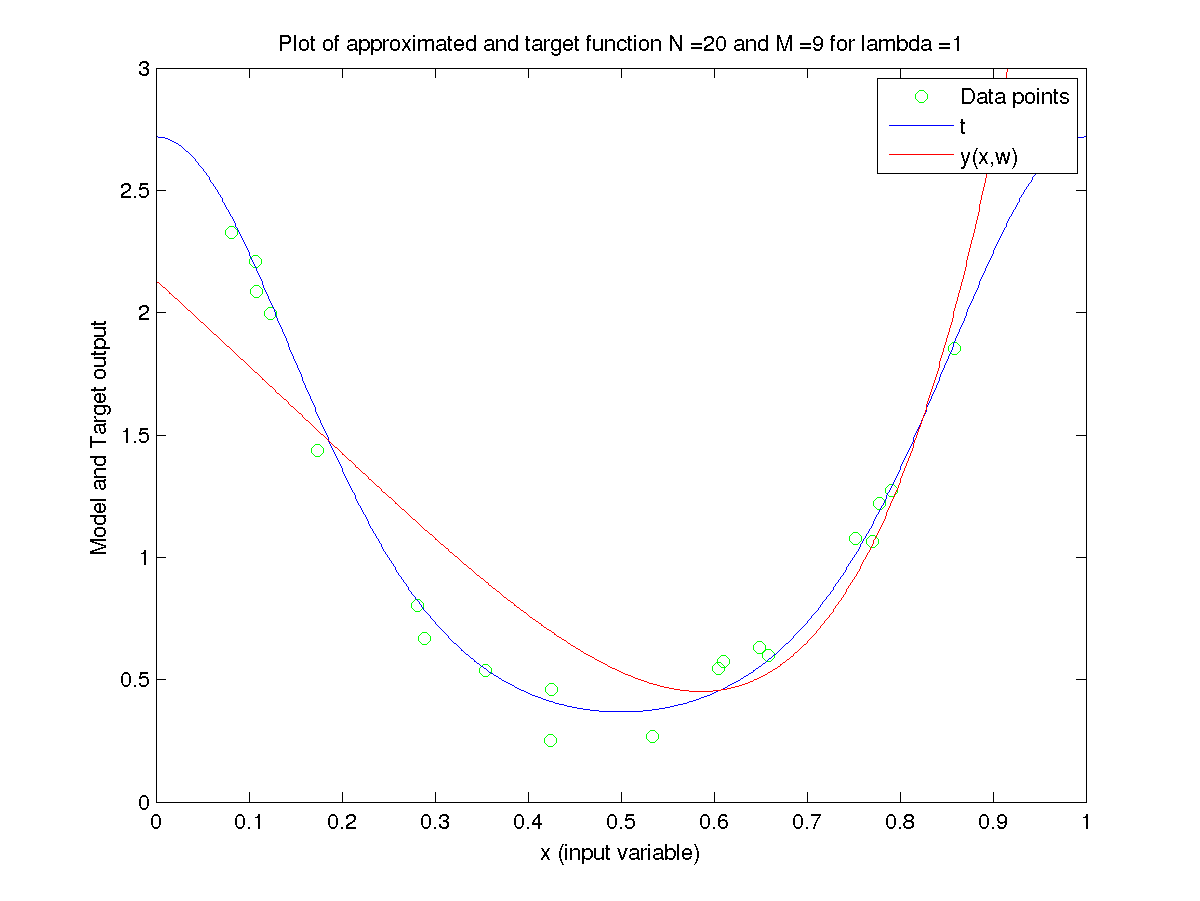
\includegraphics[width=\linewidth]{Varyinglambda_N20M9lambda1}
\caption{$\lambda$ = 1}
\end{subfigure}


\begin{subfigure}{.5\textwidth}
\centering
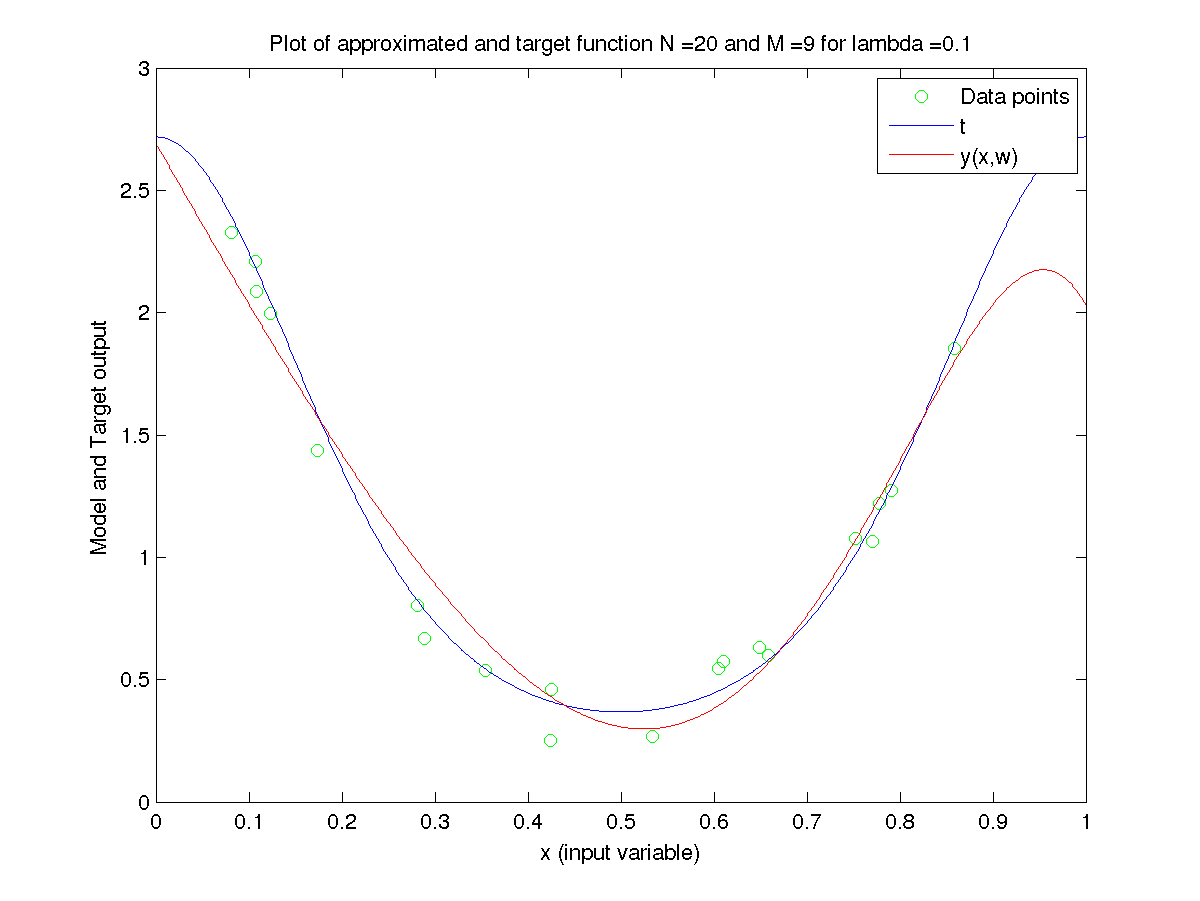
\includegraphics[width=\linewidth]{Varyinglambda_N20M9lambda01}
\caption{$\lambda$ = 0.1}
\end{subfigure}
\begin{subfigure}{.5\textwidth}
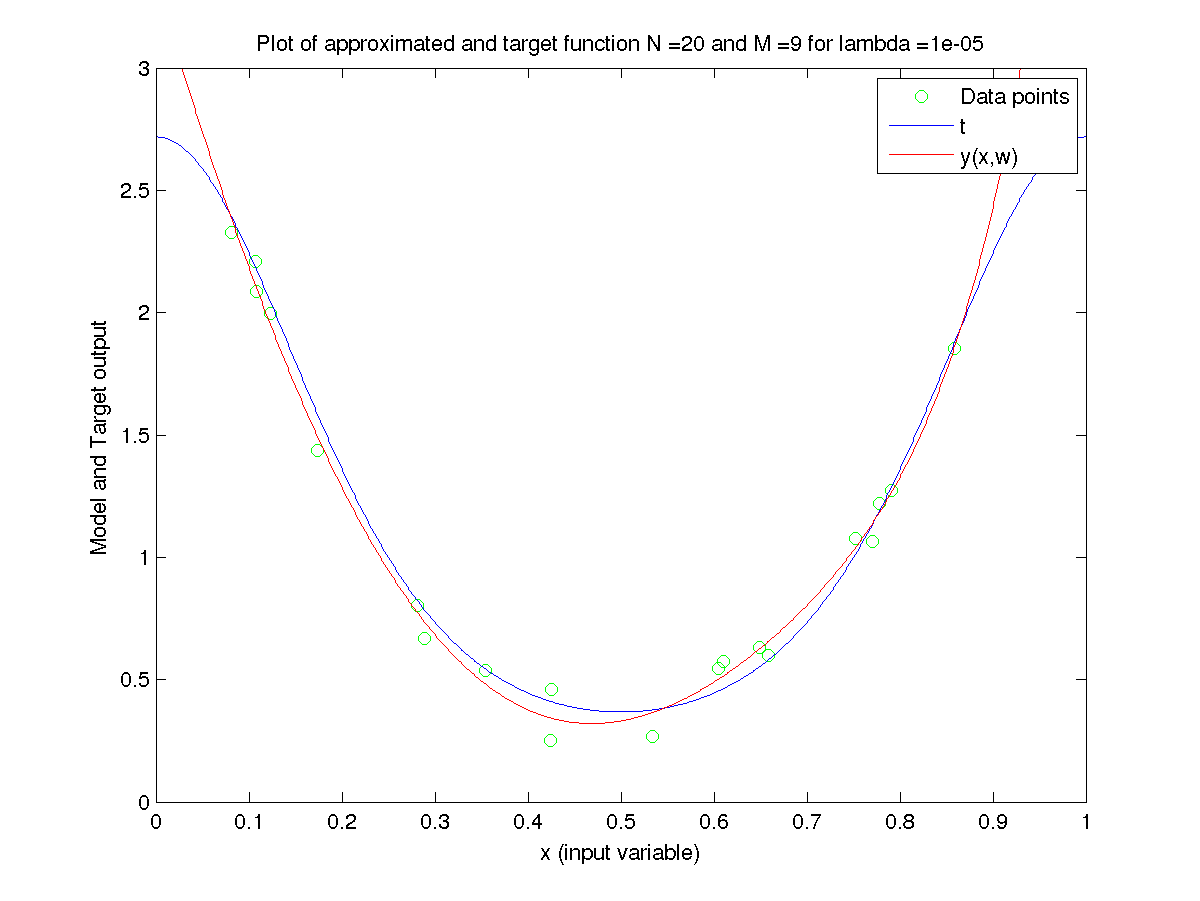
\includegraphics[width=\linewidth]{Varyinglambda_N20M9lambda1e-05}
\caption{$\lambda$ = $10^{-5}$}
\end{subfigure}



\end{figure}


\textbf{Observations: \newline}
\begin{itemize}
\item We can clearly notice the overfitting when regularization is not applied($\lambda$ = 0) in the first plot.
\item At the same time, $\lambda$ = 1 in the second plot is a very high penalization of weights again leading to a relatively poor fit since less weightage is given to the error on the training points. 
\item The third plot corresponds to $\lambda$ = 0.1. While this leads to a better fit than either of the above, it is still a high value penalization.
\item The last plot corresponds to $\lambda$ = $10^{-5}$. This provides the closest approximation to the true function among these 4 plots. Thus typically small values of $\lambda$ are investigated to minimize the overall error and produce the best fit, using the validation dataset. 
\end{itemize}
\newpage

\subsubsection{Plots of RMS Error - Question 3}
\begin{flushleft}
The following plots show the RMS Error obtained on training models of different complexities and different regularization parameters on training sets of different sizes. For each set of plots generated on varying 1 parameter (say $M$) , the optimal value of the other parameter (say $\lambda$) is obtained by cross-validation. 
The errors have been shown on all 3 datasets for each case (test, train and validation). The plots for 20 size training set undergo lot of variation for every new sampling due to the small size of the dataset, and have been added only for the sake of completion.
\end{flushleft}

\begin{figure}[H]

\begin{subfigure}{.5\textwidth}
\centering
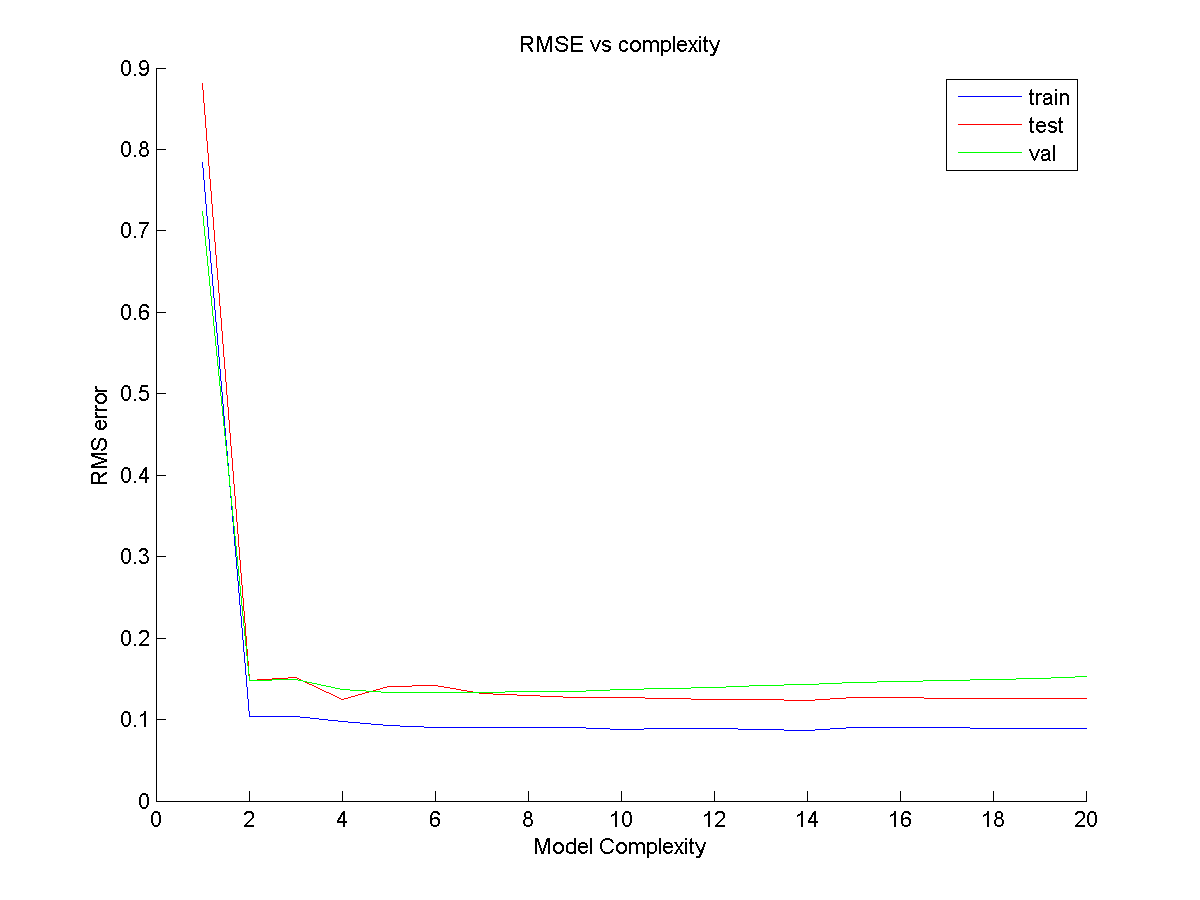
\includegraphics[width=\linewidth]{RMS_complexity_20}
\caption{Varying M, Optimal $\lambda$, 20 train size}
\end{subfigure}
\begin{subfigure}{.5\textwidth}
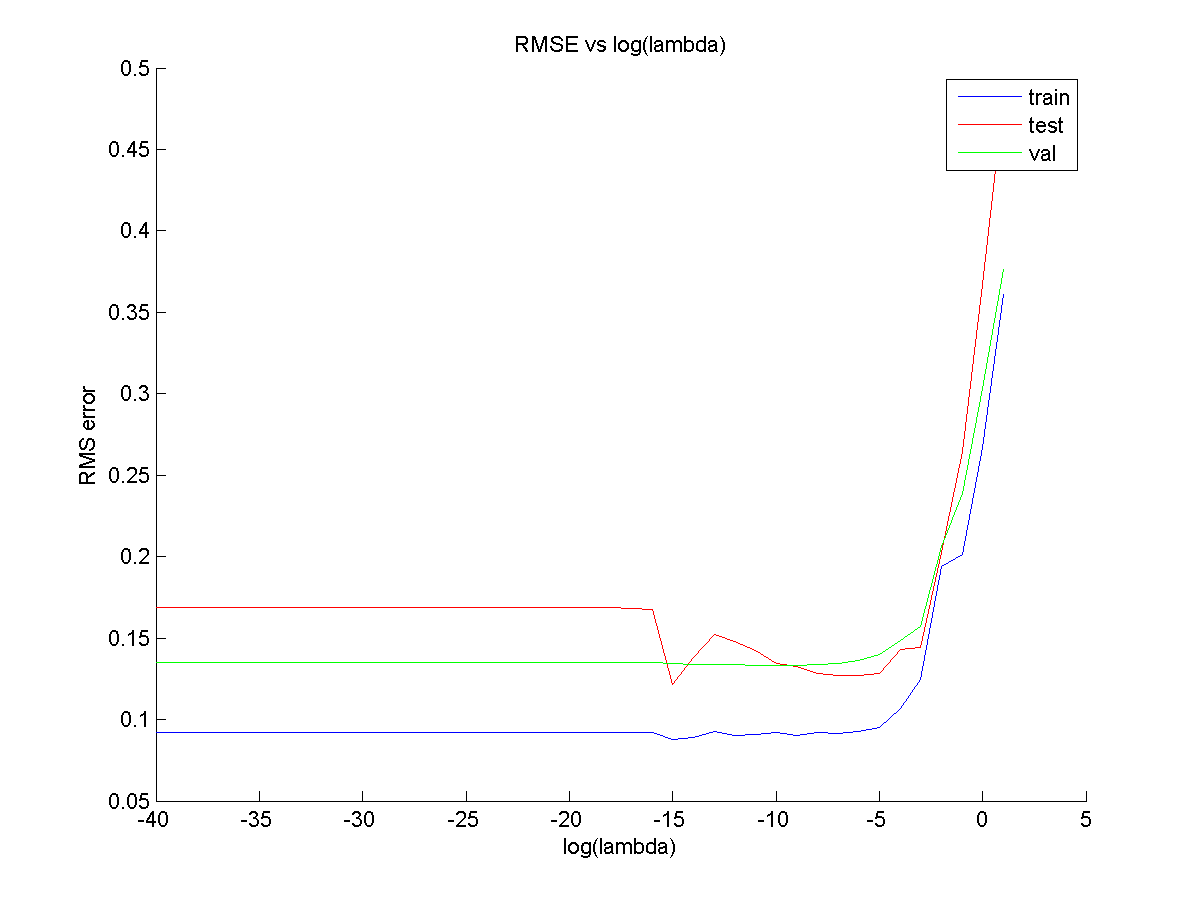
\includegraphics[width=\linewidth]{RMS_lambda_20}
\caption{Optimal M, Varying $\lambda$, 20 train size}
\end{subfigure}


\begin{subfigure}{.5\textwidth}
\centering
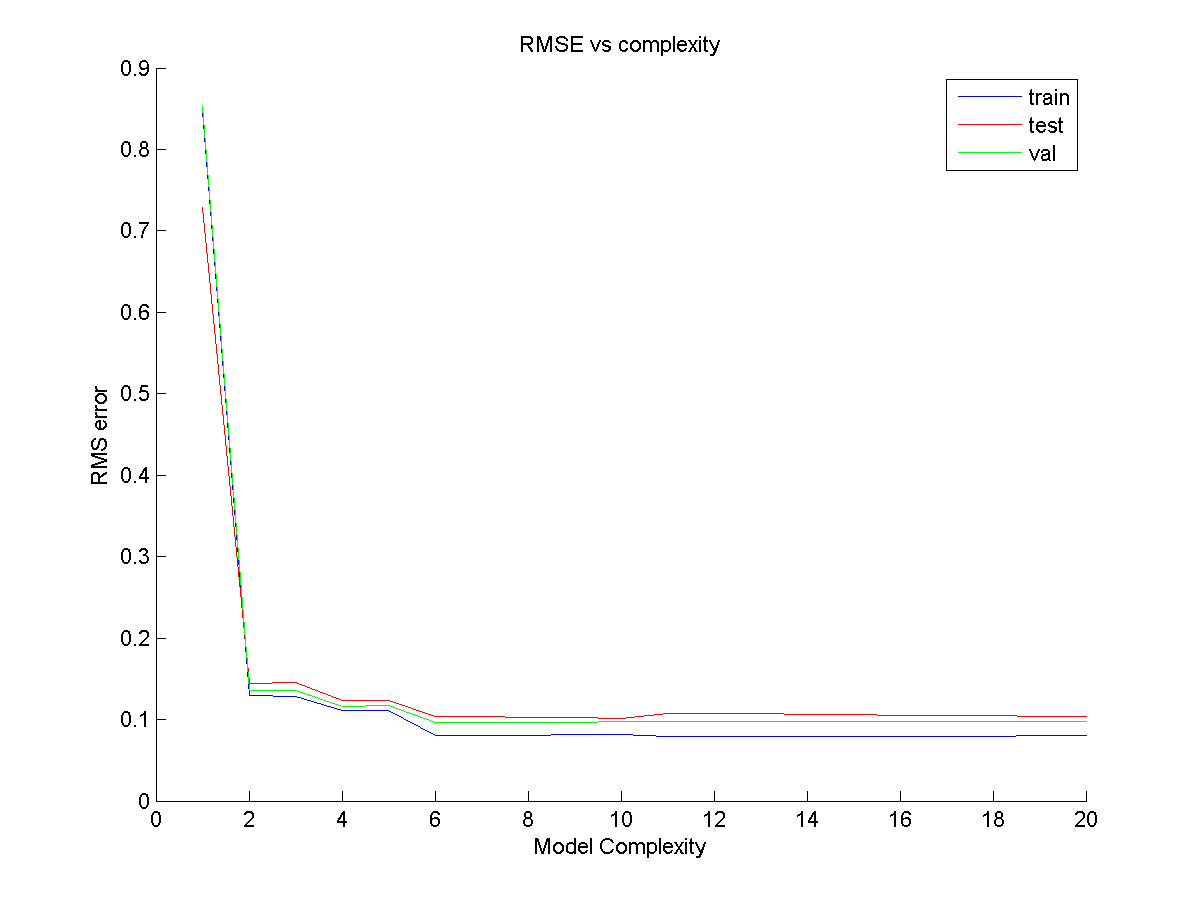
\includegraphics[width=\linewidth]{RMS_complexity_100}
\caption{Varying M, Optimal $\lambda$, 100 train size}
\end{subfigure}
\begin{subfigure}{.5\textwidth}
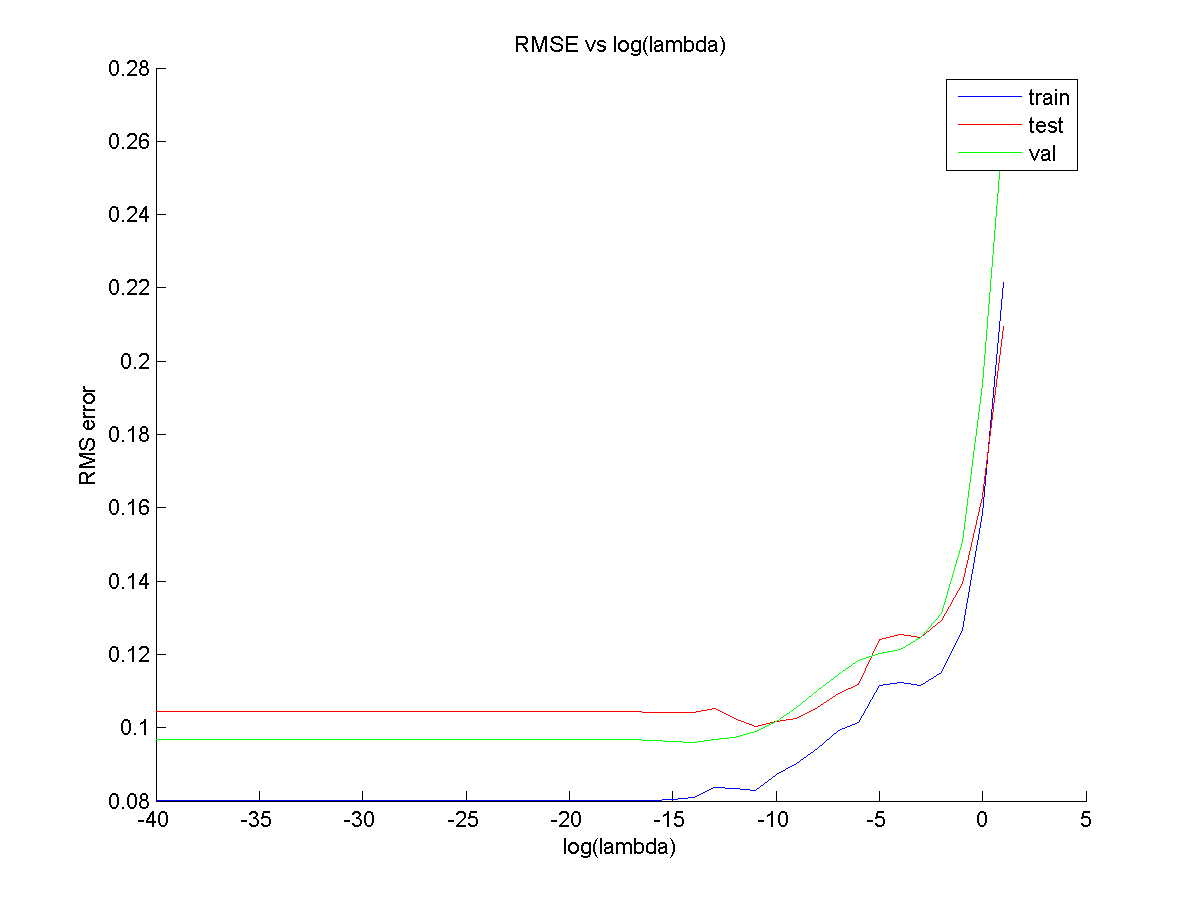
\includegraphics[width=\linewidth]{RMS_lambda_100}
\caption{Optimal M, Varying $\lambda$, 100 train size}
\end{subfigure}

\begin{subfigure}{.5\textwidth}
\centering
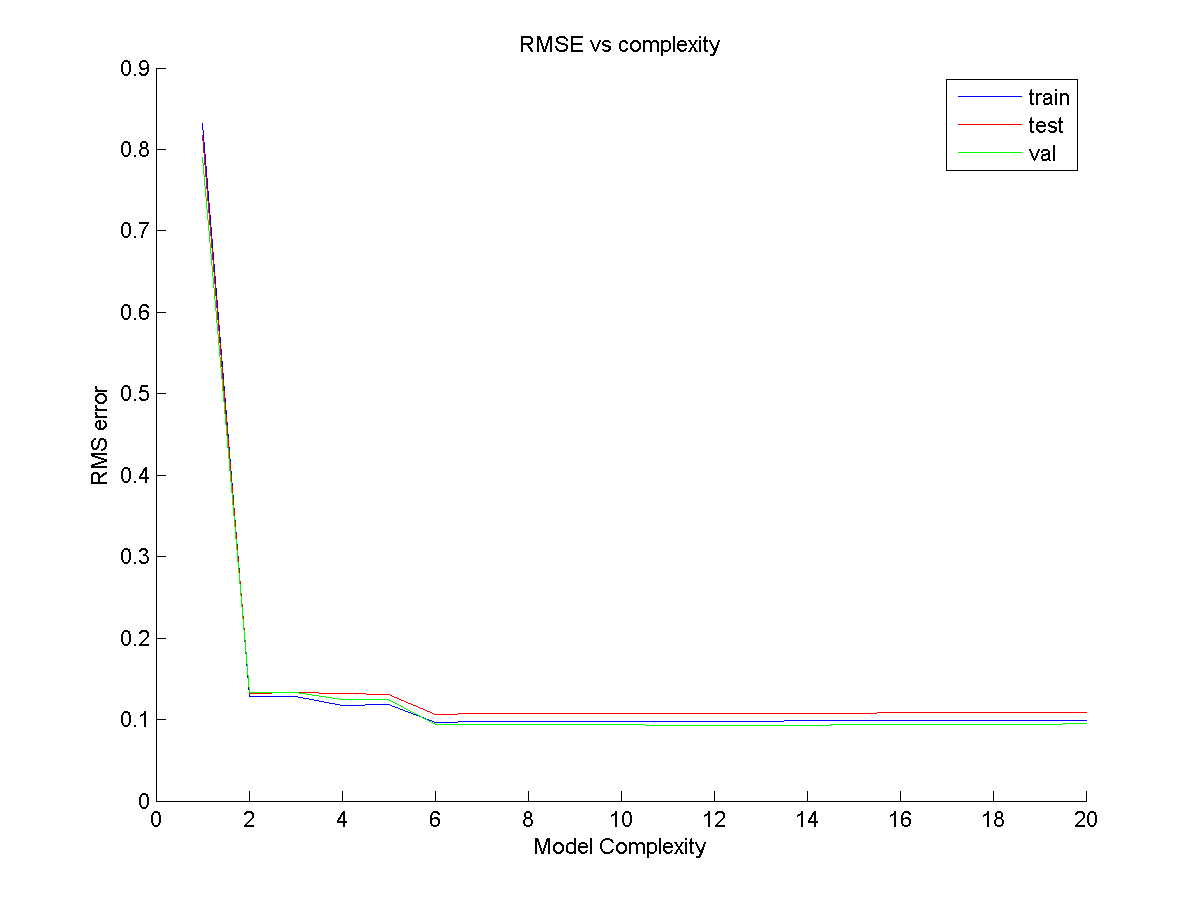
\includegraphics[width=\linewidth]{RMS_complexity_1000}
\caption{Varying M, Optimal $\lambda$, 1000 train size}
\end{subfigure}
\begin{subfigure}{.5\textwidth}
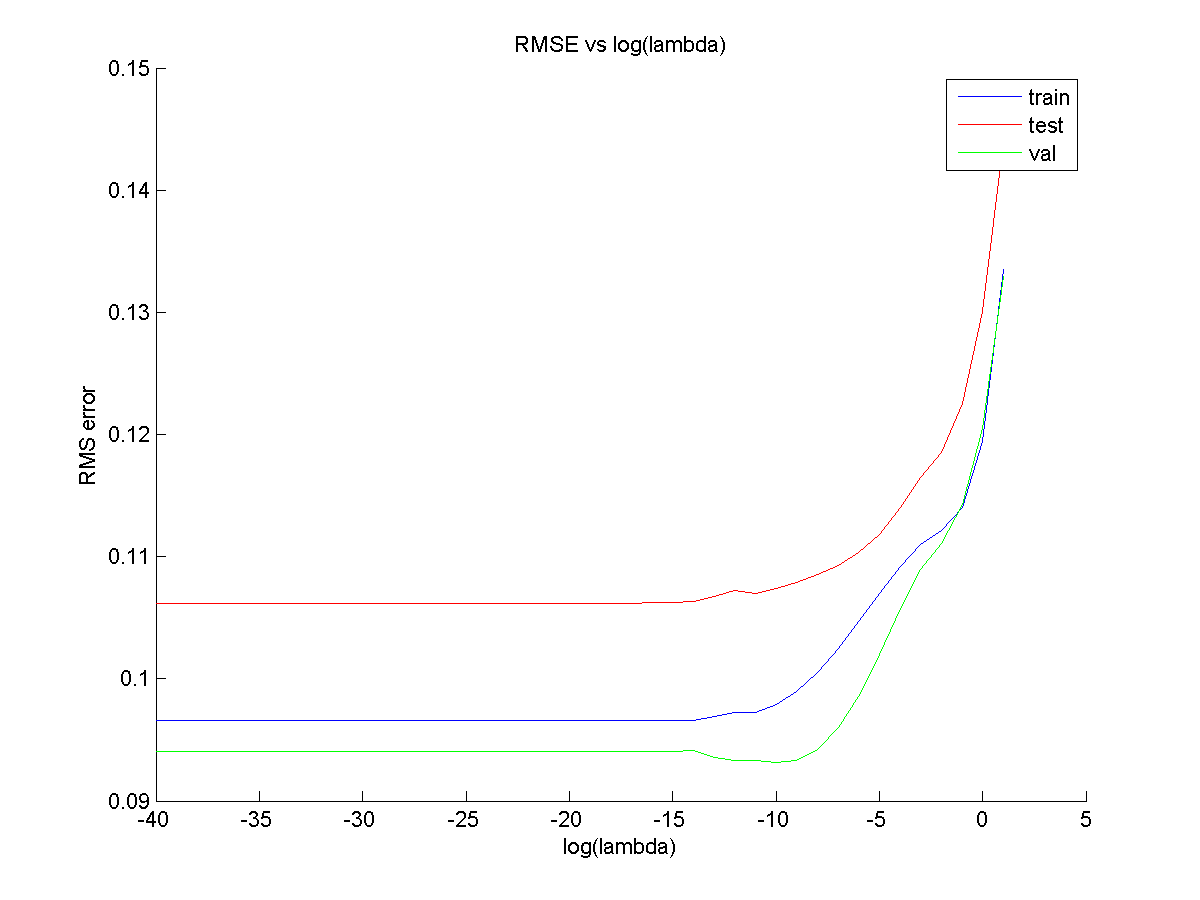
\includegraphics[width=\linewidth]{RMS_lambda_1000}
\caption{Optimal M, Varying $\lambda$, 1000 train size}
\end{subfigure}

\end{figure}

\subsubsection{Scatter plots of target and model output}
The plots obtained here, have been generated in a process similar to that of question 1. 
The following plots show the scatter plots on the training data obtained on varying the degree of the polynomial $M$ for training dataset size $N = 20$.

\begin{figure}[H]

\begin{subfigure}{.5\textwidth}
\centering
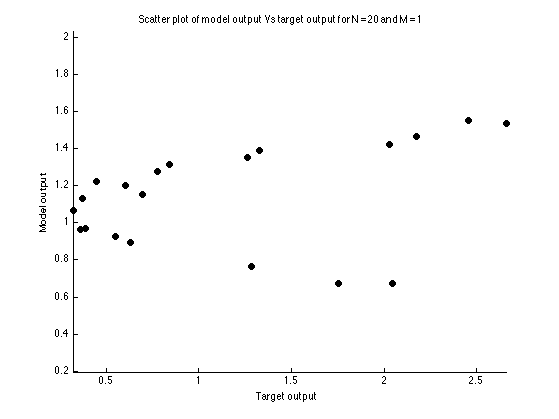
\includegraphics[width=\linewidth]{Scatter_1/VaryingM_N20M1}
\caption{N = 20 M = 1}
\end{subfigure}
\begin{subfigure}{.5\textwidth}
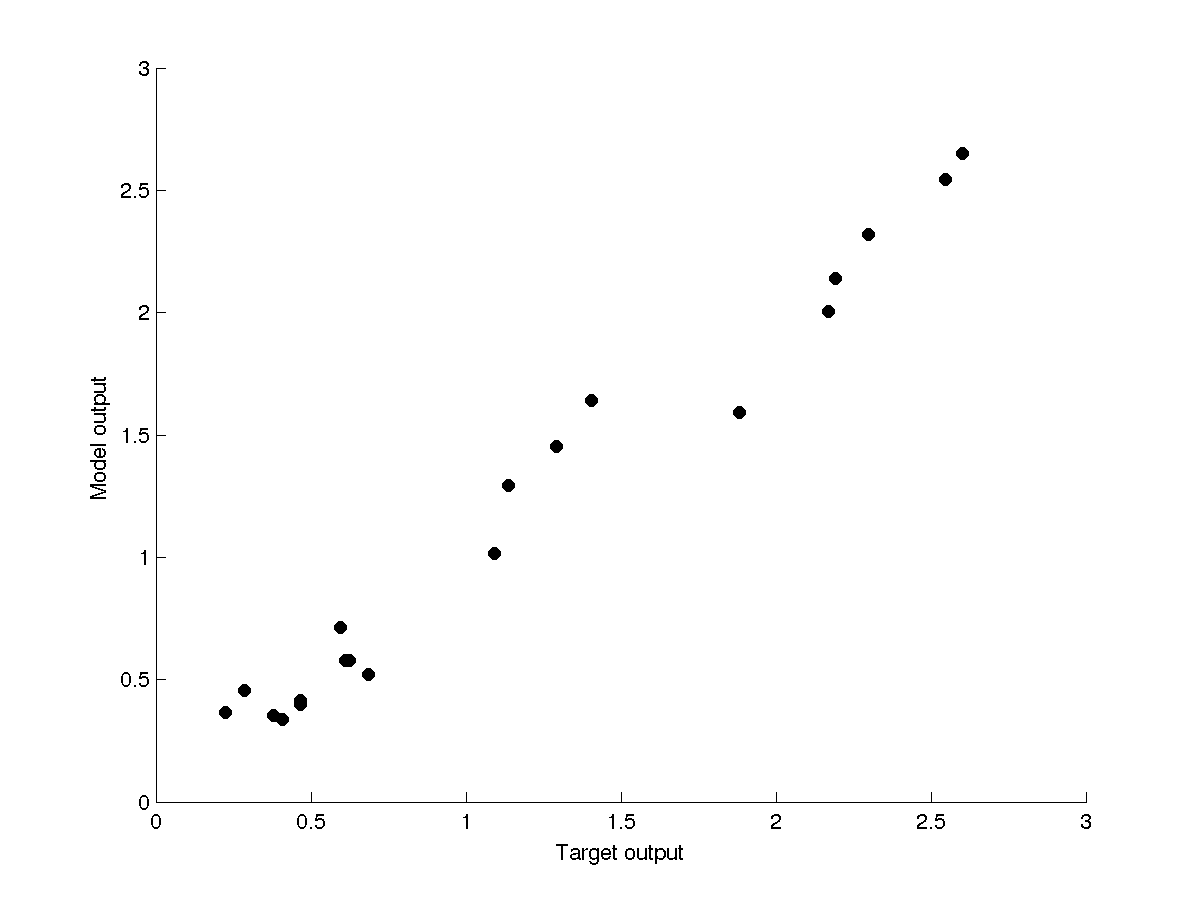
\includegraphics[width=\linewidth]{Scatter_1/VaryingM_N20M3}
\caption{N = 20 M = 3}
\end{subfigure}


\begin{subfigure}{.5\textwidth}
\centering
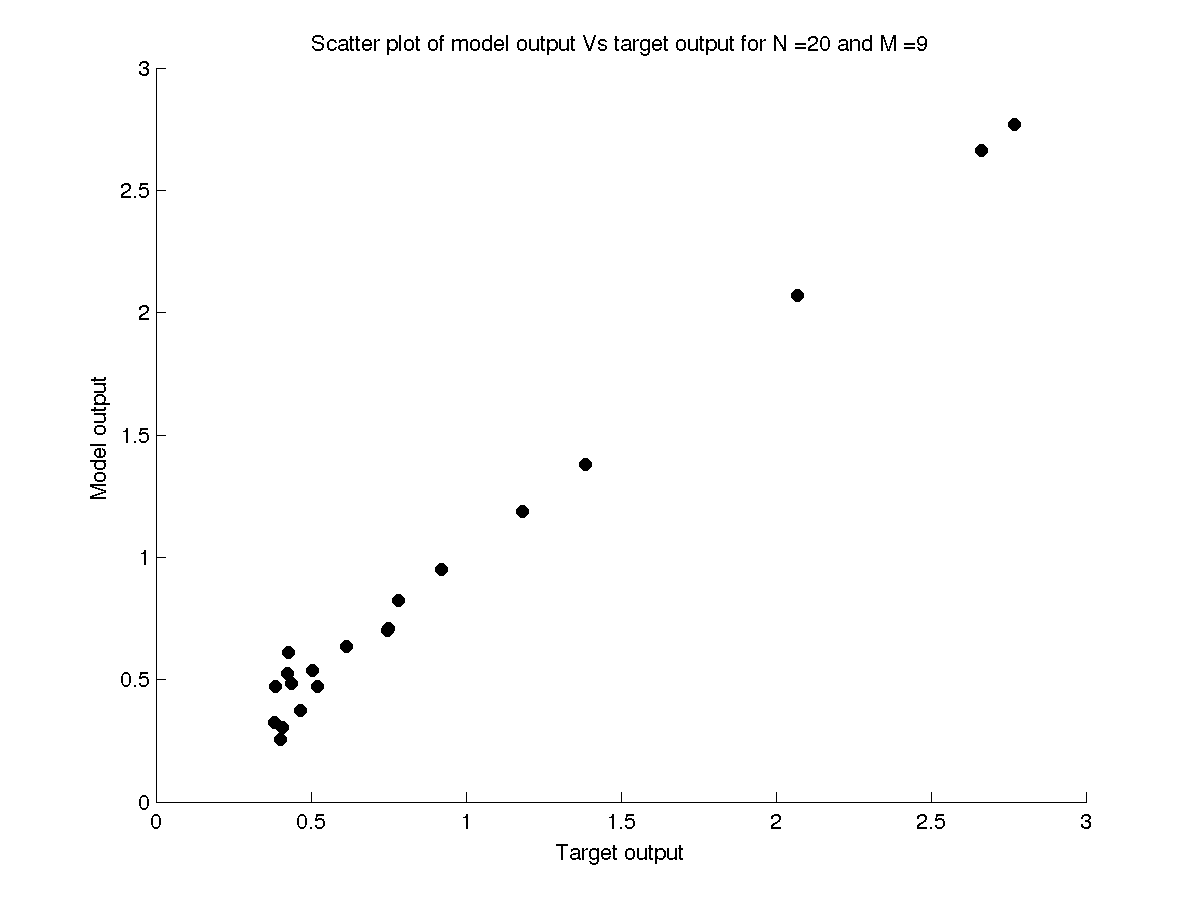
\includegraphics[width=\linewidth]{Scatter_1/VaryingM_N20M9}
\caption{N = 20 M = 9}
\end{subfigure}
\begin{subfigure}{.5\textwidth}
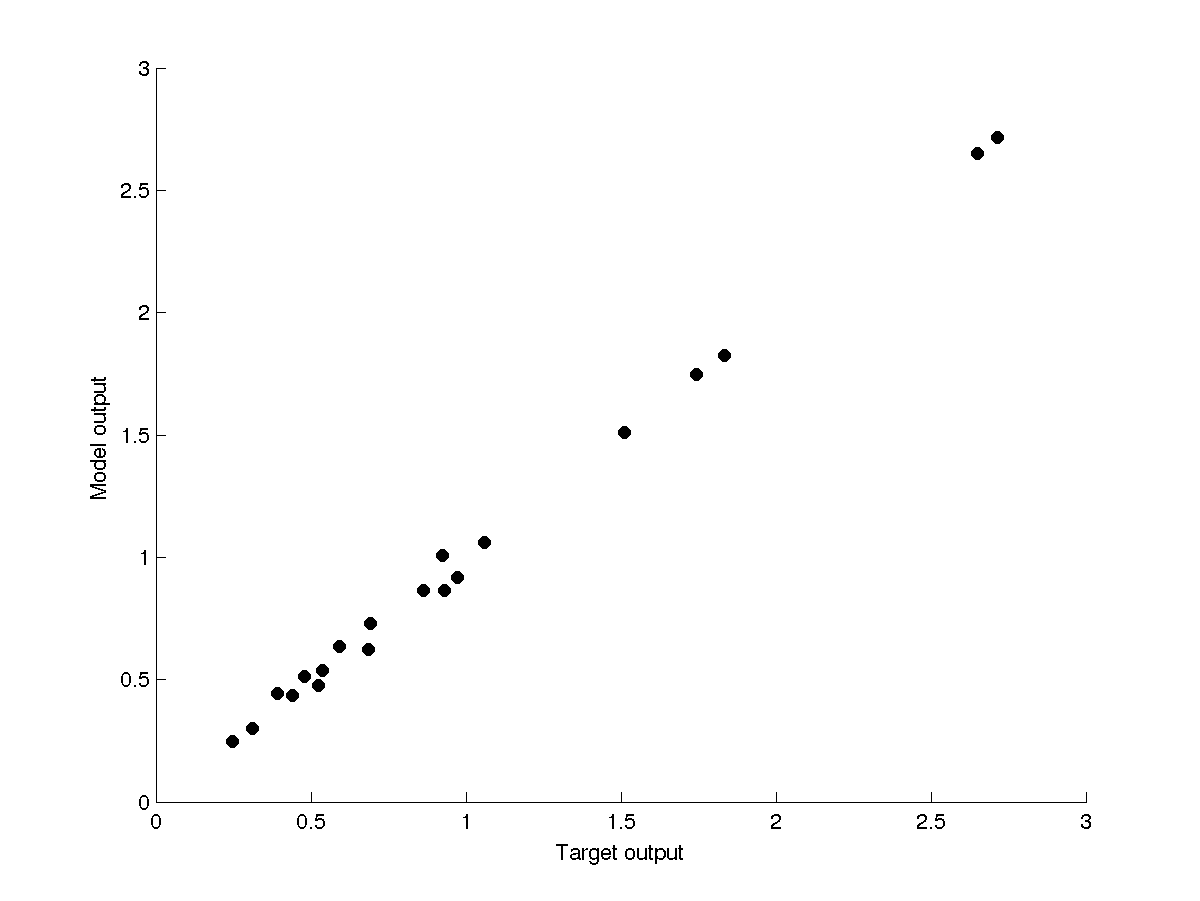
\includegraphics[width=\linewidth]{Scatter_1/VaryingM_N20M15}
\caption{N = 20 M = 15}
\end{subfigure}


\end{figure}

\textbf{Observations : \newline}
\begin{itemize}
\item In case of a scatter plot, we would ideally like the points to lie along the $y = x$ line. 
\item We observe that for $M=1$, we get a bad fit to the data, which leads to a bad plot.
\item $M = 3$ does better, while $M=9$ and 15 do much better as they fit the training data too well, leading to nearly perfect plots. This is because of overfitting to the training data, which leads to model output being very close to the target output, though the generalization ability is bad.

\end{itemize}

The next set of scatter plots show the variation w.r.t the training set size $N$, namely $N = 100, 1000$.

\begin{figure}[H]

\begin{subfigure}{.5\textwidth}
\centering
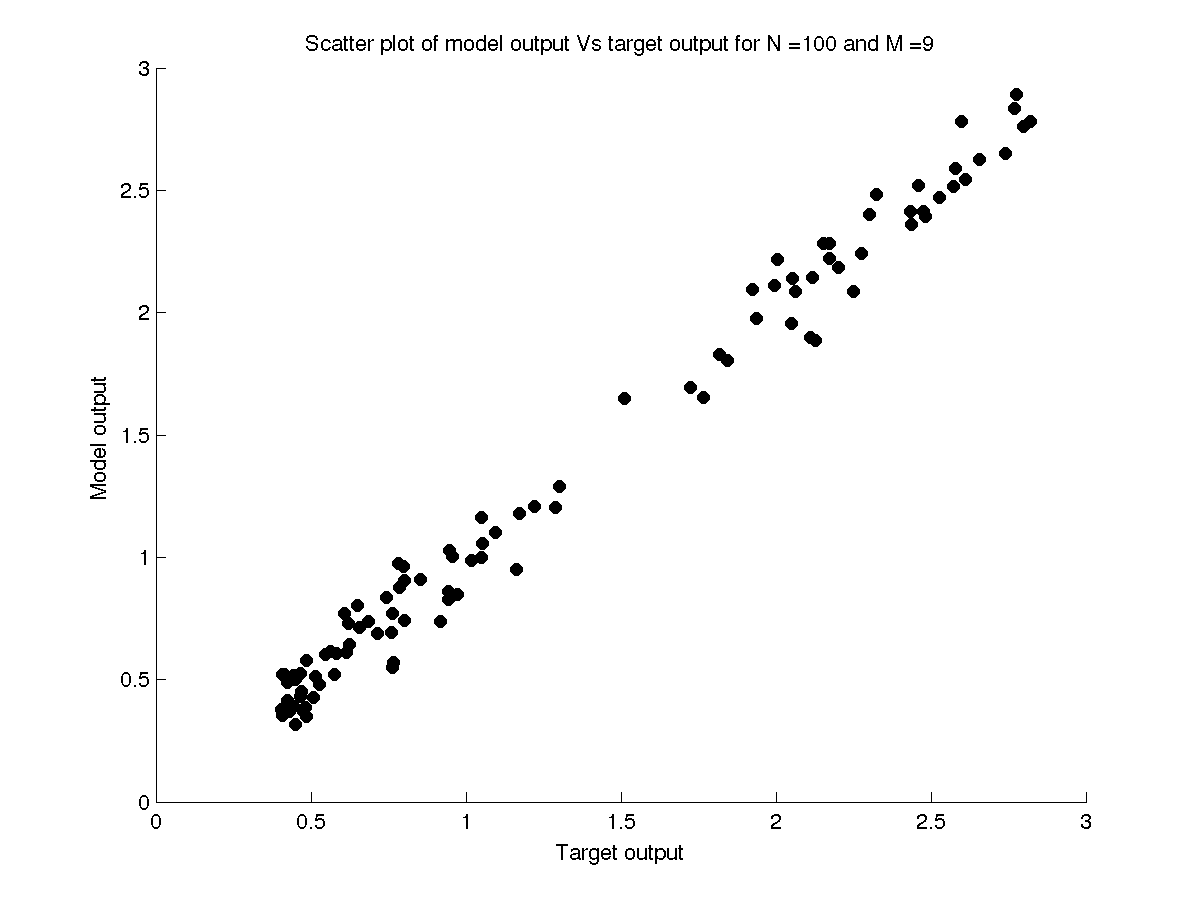
\includegraphics[width=\linewidth]{Scatter_1/VaryingN_N100M9}
\caption{N = 100 M = 9}
\end{subfigure}
\begin{subfigure}{.5\textwidth}
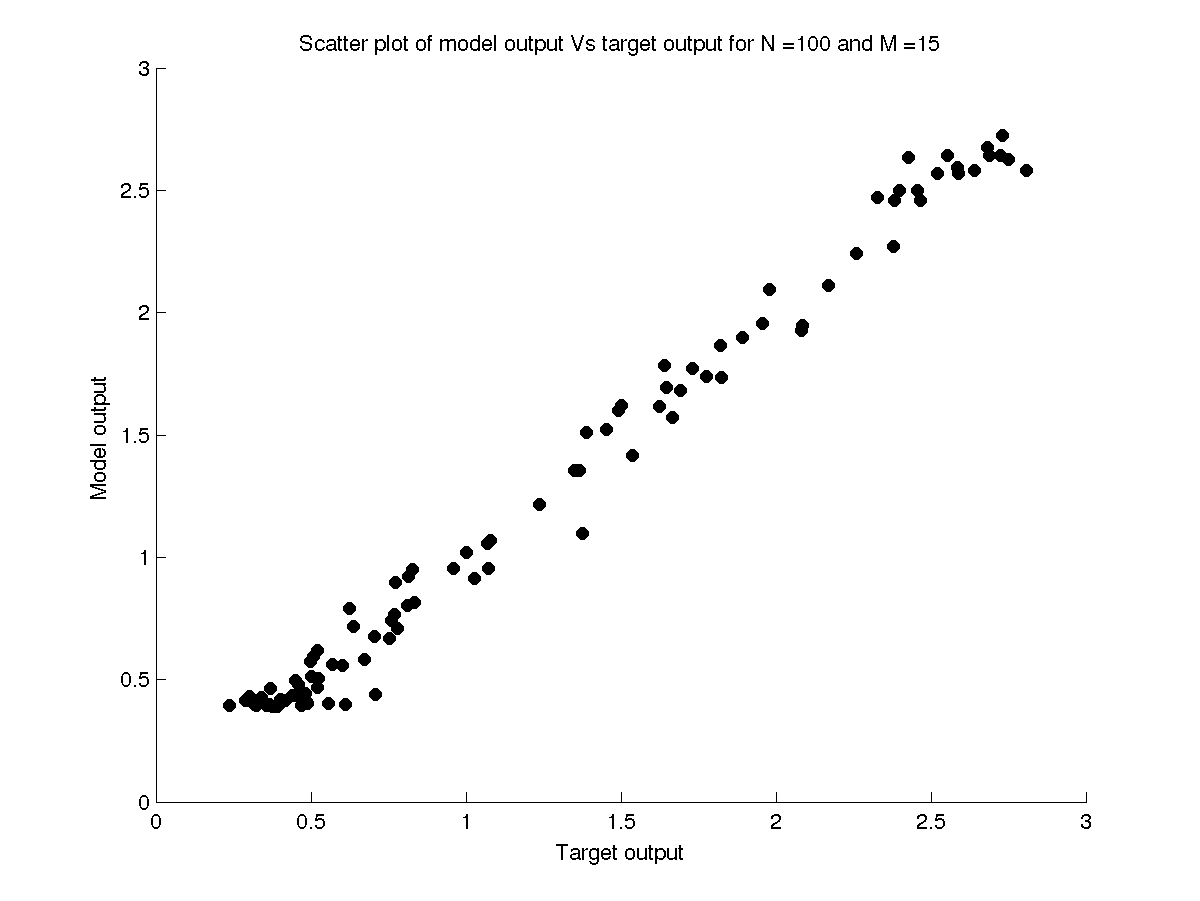
\includegraphics[width=\linewidth]{Scatter_1/VaryingN_N100M15}
\caption{N = 100 M = 15}
\end{subfigure}


\begin{subfigure}{.5\textwidth}
\centering
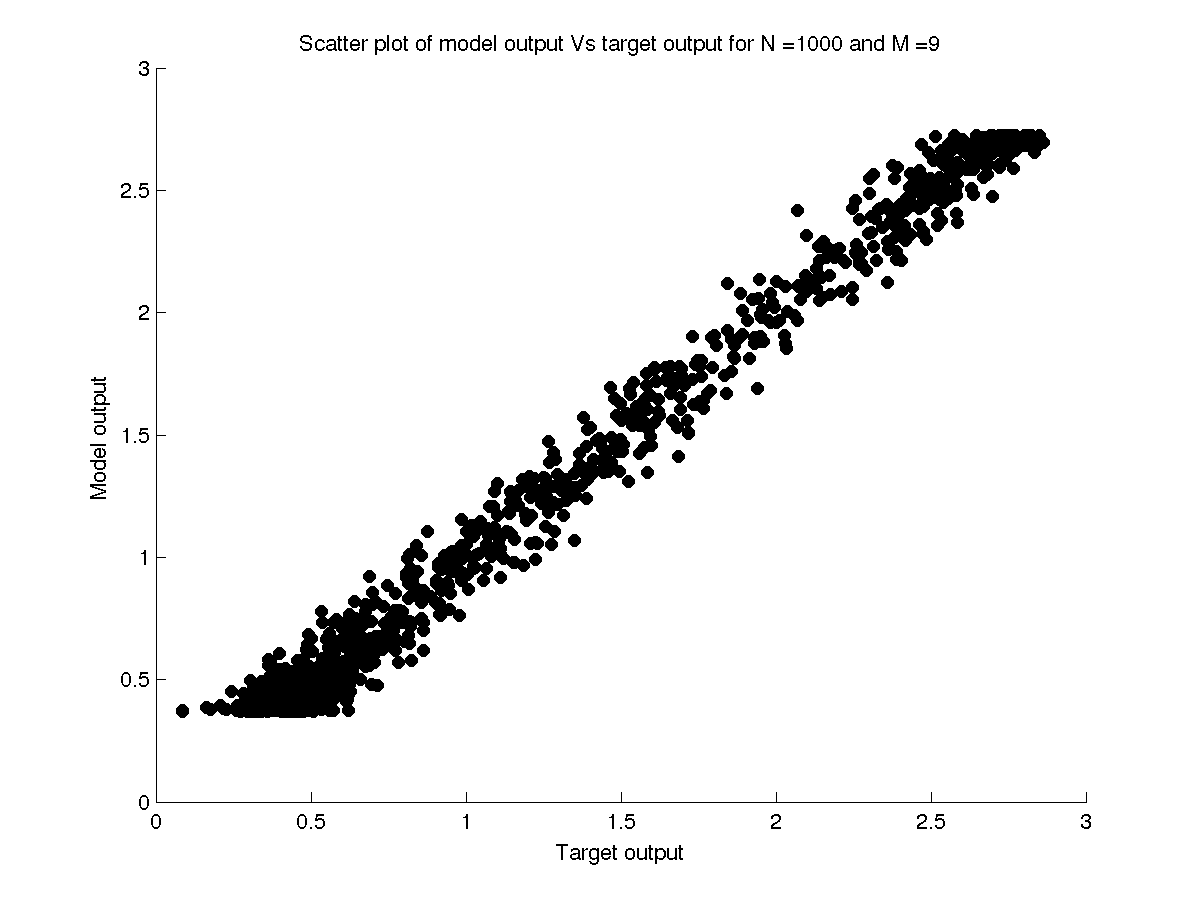
\includegraphics[width=\linewidth]{Scatter_1/VaryingN_N1000M9}
\caption{N = 1000 M = 9}
\end{subfigure}
\begin{subfigure}{.5\textwidth}
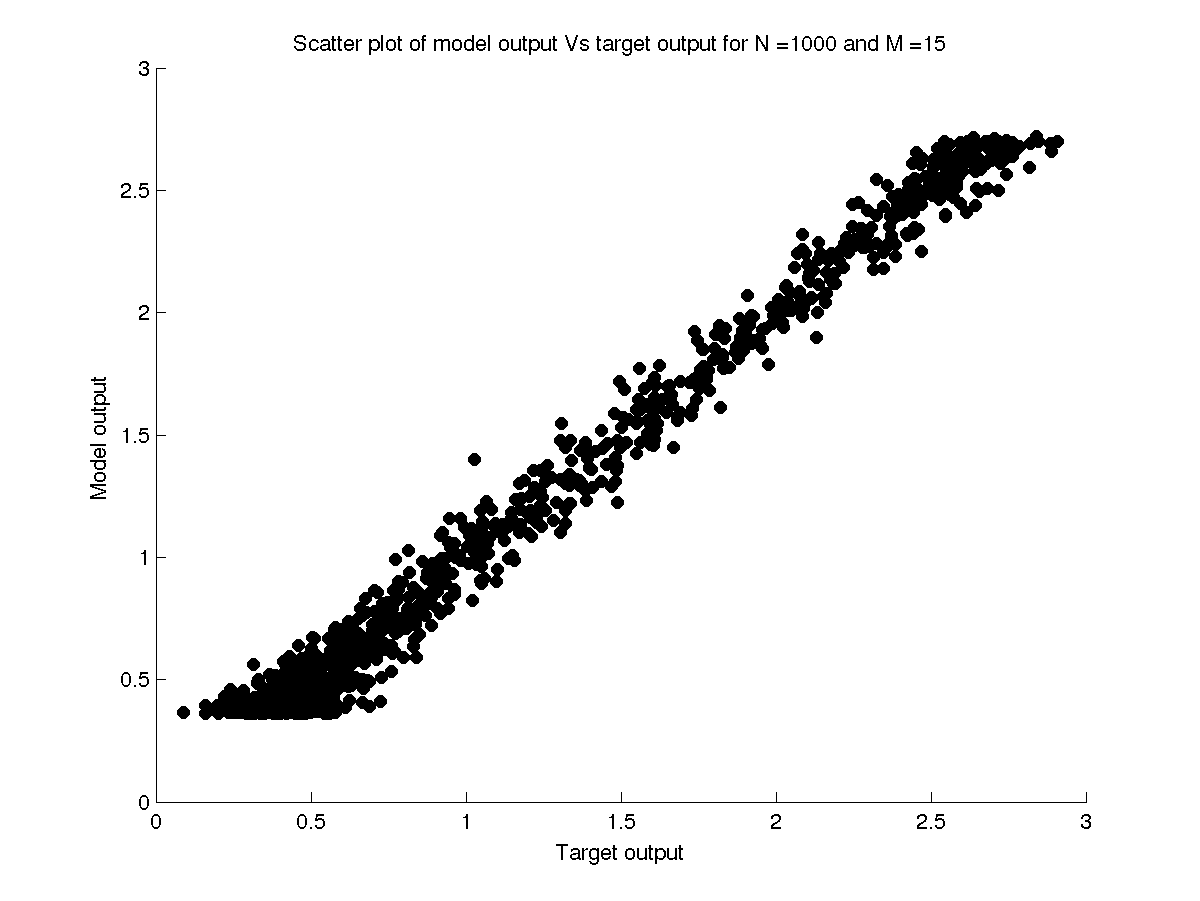
\includegraphics[width=\linewidth]{Scatter_1/VaryingN_N1000M15}
\caption{N = 1000 M = 15}
\end{subfigure}



\end{figure}


\textbf{Observations : \newline}
\begin{itemize}
\item For $M=9$, we can see that both of the models ($N = 100 ,1000$) perform well, as we have sufficient number of training examples to build a good model.
\item Again for $M = 15$, we see that both models seem to give good results on the training data. Actually, overfitting happens in the case of $N= 100, M = 15$. To see this, we look at the scatter plots obtained on the test data below for the same model complexity $M = 15$.
\item We can that the generalization ability is more, when we have a greater number of training examples, as exemplified by the better plot obtained when 1000 training examples are used. As we have overfitting when $N = 100, M = 15$, the model output doesn't follow the target output closely. 

\item Next, the effect of $\lambda$ is analyzed.
\end{itemize}

\begin{figure}[H]

\begin{subfigure}{.5\textwidth}
\centering
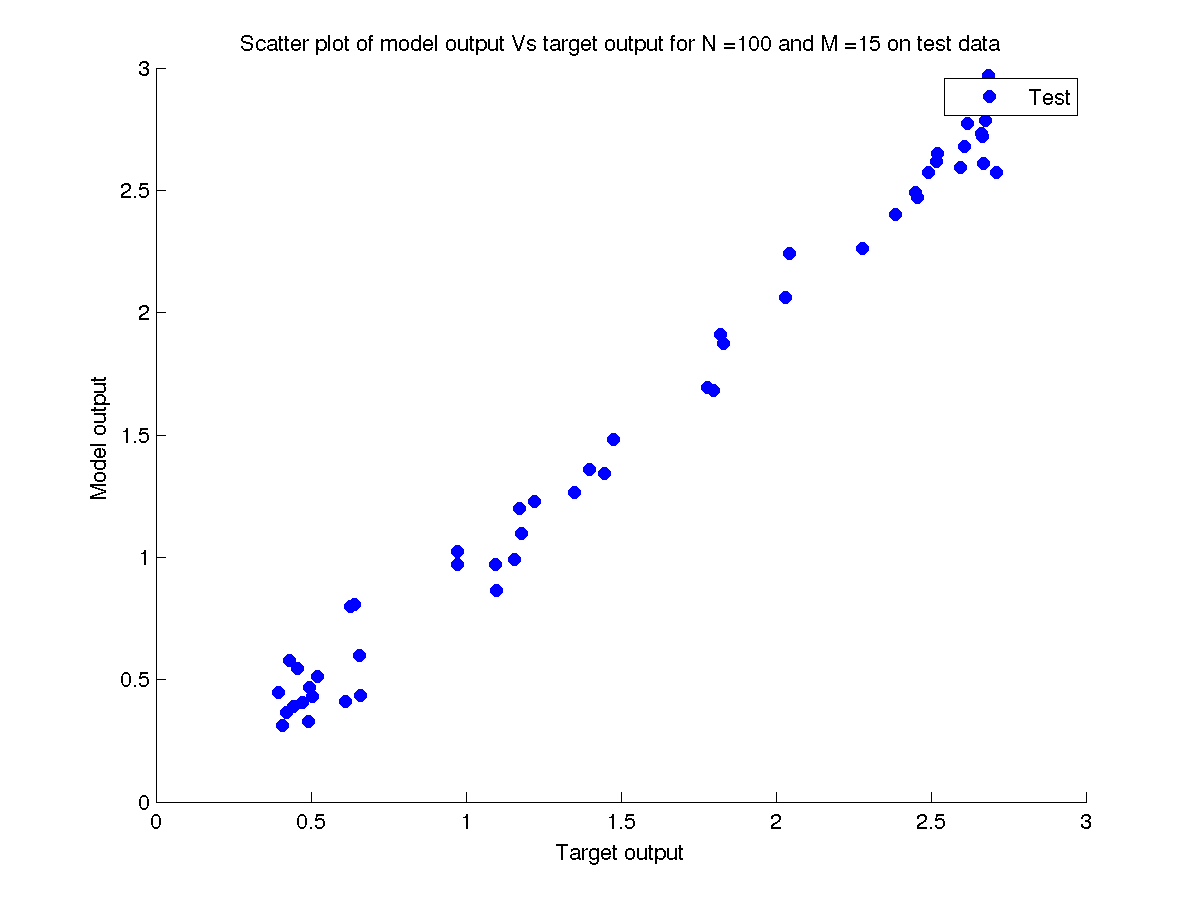
\includegraphics[width=\linewidth]{Scatter_1/VaryingN_N100M15_test}
\caption{N = 100 M = 15}
\end{subfigure}
\begin{subfigure}{.5\textwidth}
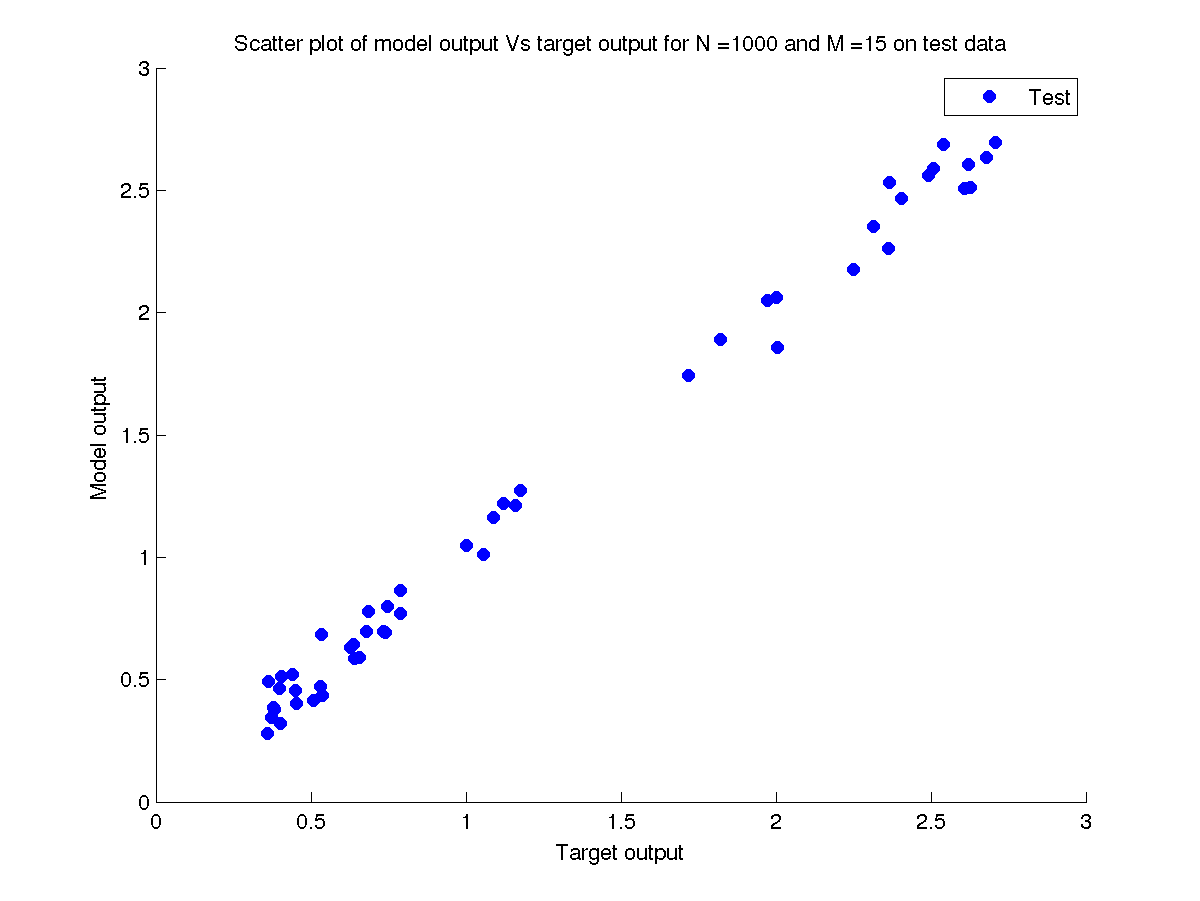
\includegraphics[width=\linewidth]{Scatter_1/VaryingN_N1000M15_test}
\caption{N = 1000 M = 15}
\end{subfigure}

\end{figure}



The plots below show the scatter plots obtained on varying $\lambda$, for $N = 20$ and $M = 9$. The results obtained were very similar to that of question 1.\newline



\begin{figure}[H]

\begin{subfigure}{.5\textwidth}
\centering
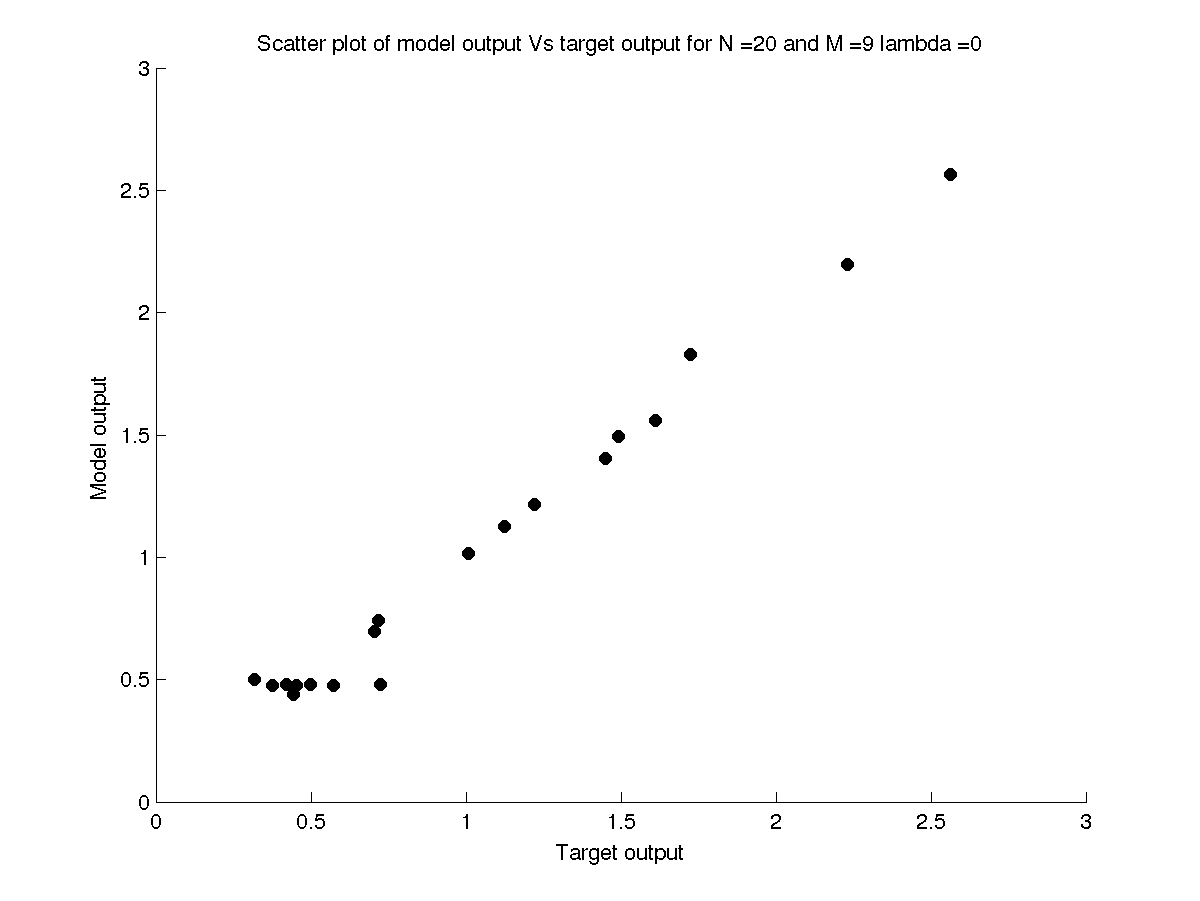
\includegraphics[width=\linewidth]{Scatter_1/Varyinglambda_N20M9lambda0}
\caption{$\lambda$ = 0}
\end{subfigure}
\begin{subfigure}{.5\textwidth}
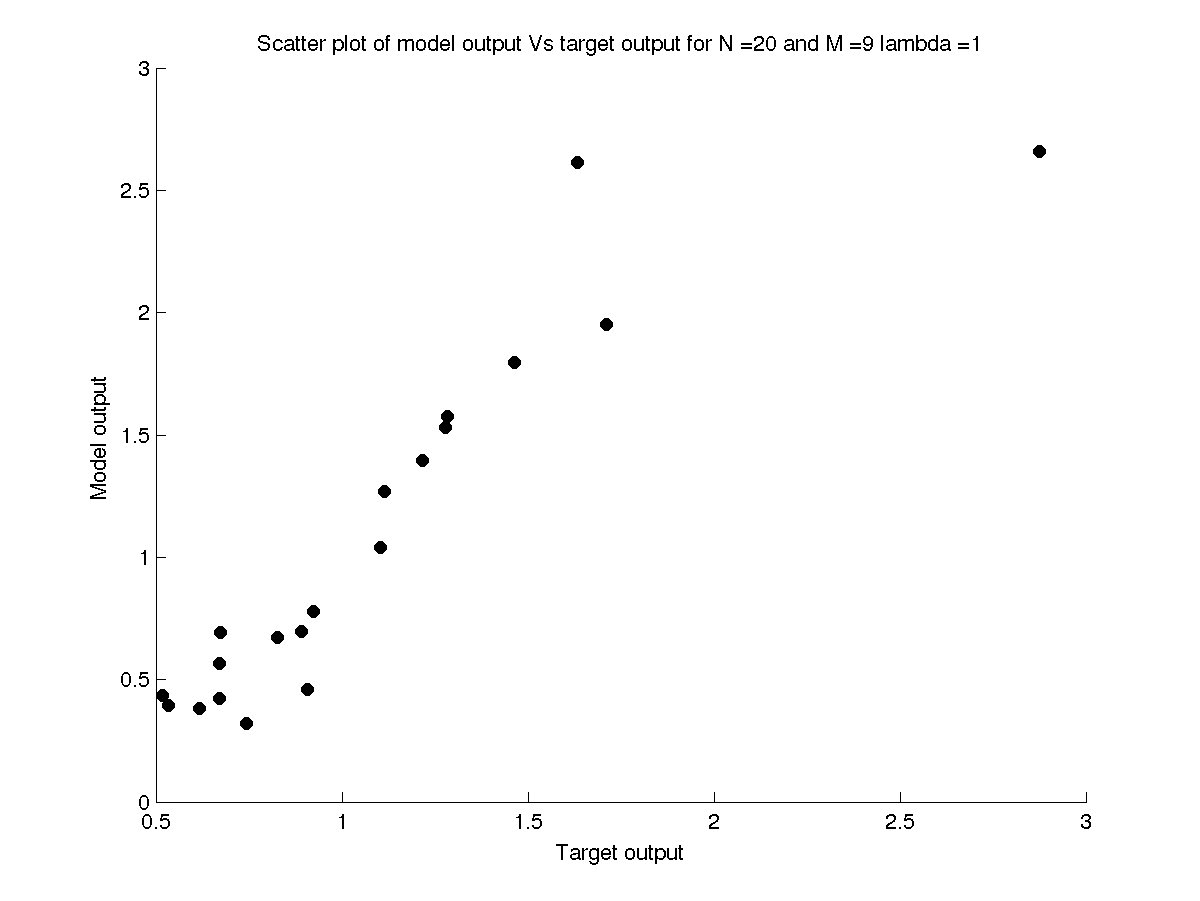
\includegraphics[width=\linewidth]{Scatter_1/Varyinglambda_N20M9lambda1}
\caption{$\lambda$ = 1}
\end{subfigure}


\begin{subfigure}{.5\textwidth}
\centering
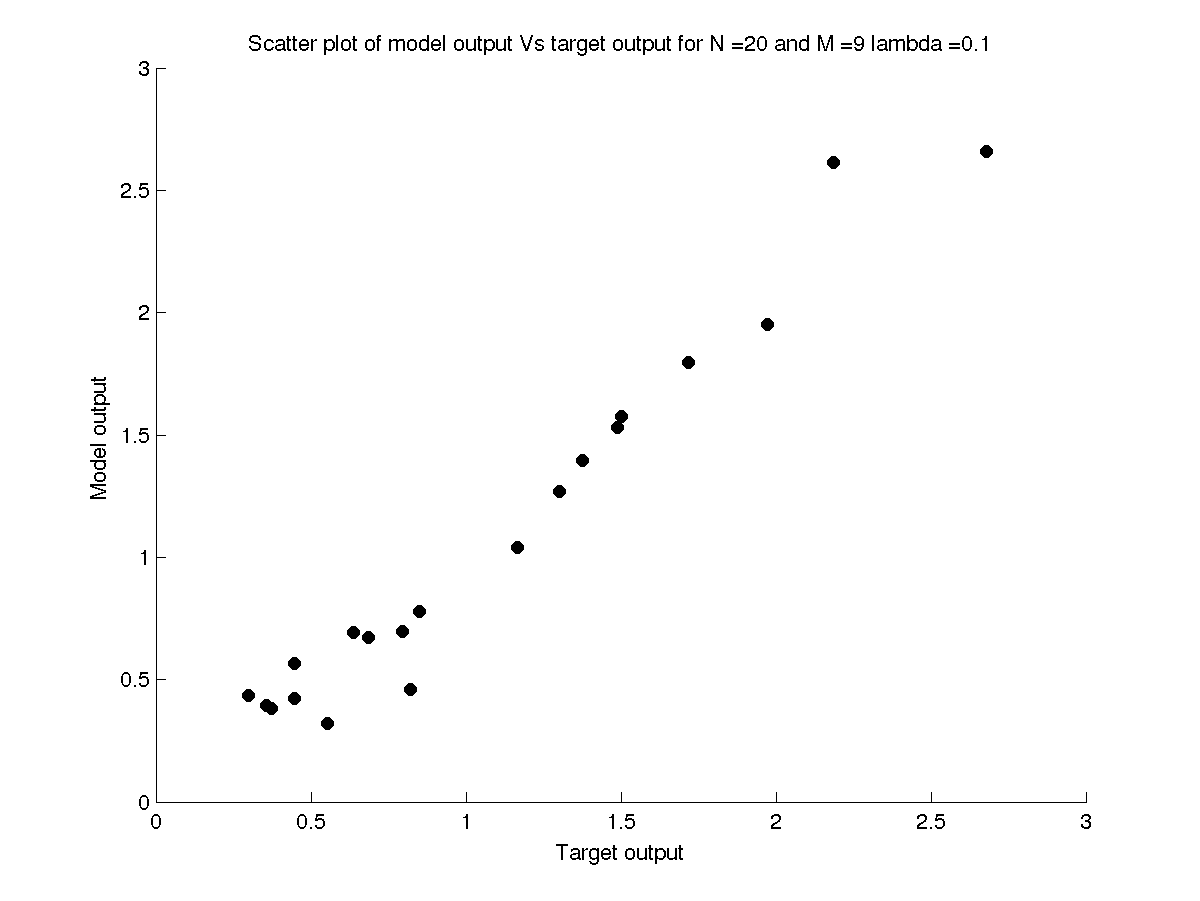
\includegraphics[width=\linewidth]{Scatter_1/Varyinglambda_N20M9lambda01}
\caption{$\lambda$ = 0.1}
\end{subfigure}
\begin{subfigure}{.5\textwidth}
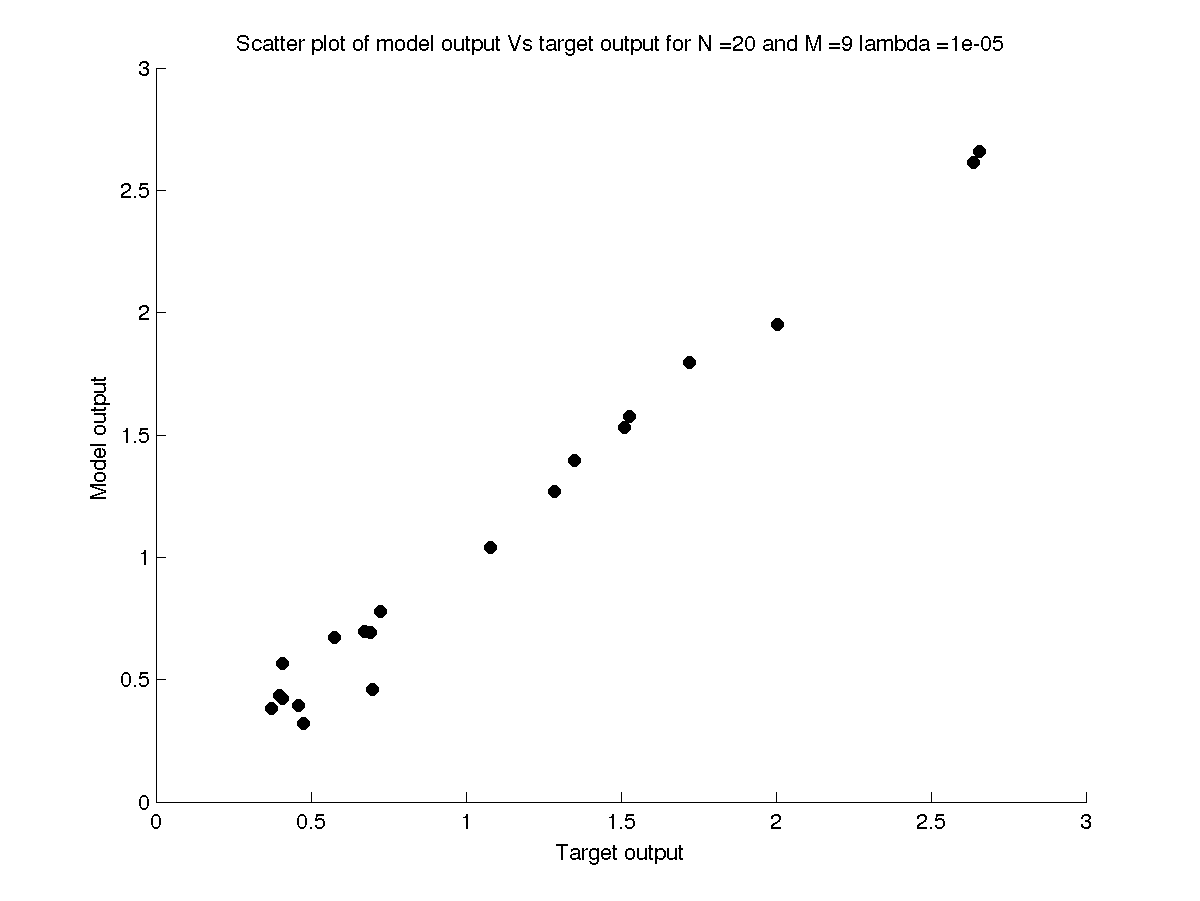
\includegraphics[width=\linewidth]{Scatter_1/Varyinglambda_N20M9lambda1e-05}
\caption{$\lambda$ = $10^{-5}$}
\end{subfigure}



\end{figure}

\textbf{Observations :}
\begin{itemize}
\item Clearly, the first plot is the case where $\lambda = 0$, i.e. no regularization.
\item Again for $\lambda = 1$, there is a very high penalization of weights leading to a bad scatter plot, while $\lambda = 0.1$ performs better.

\item The last plot corresponds to $\lambda = 10^{-5}$, which gives a good scatter plot where the model output follows the target output closely and also gives a good generalization on test examples.
\end{itemize}

\section{Dataset 2}

\subsection{Generation}
Here, we are given the dataset which is bivariate (2 input variables and 1 output variable). 3 different training sets are present, of sizes 20, 100 and 1000. The test and validation sets are of size 200 and 300 respectively.
\subsection{Model creation}

TODO - Do we need to put formulas ?


\subsection{Results}


\subsection{Surface Plots of approximated functions - Question 2}
\begin{flushleft}
The Surface plots depict the variation of the surface fit obtained on varying the model complexity ($M$ - No. of basis functions), on the training dataset of size 100. Each plot shows the data points and the fitted surface obtained by linear model of regression on Gaussian Basis functions.

\end{flushleft}
\begin{figure}[H]

\begin{subfigure}{.5\textwidth}
\centering
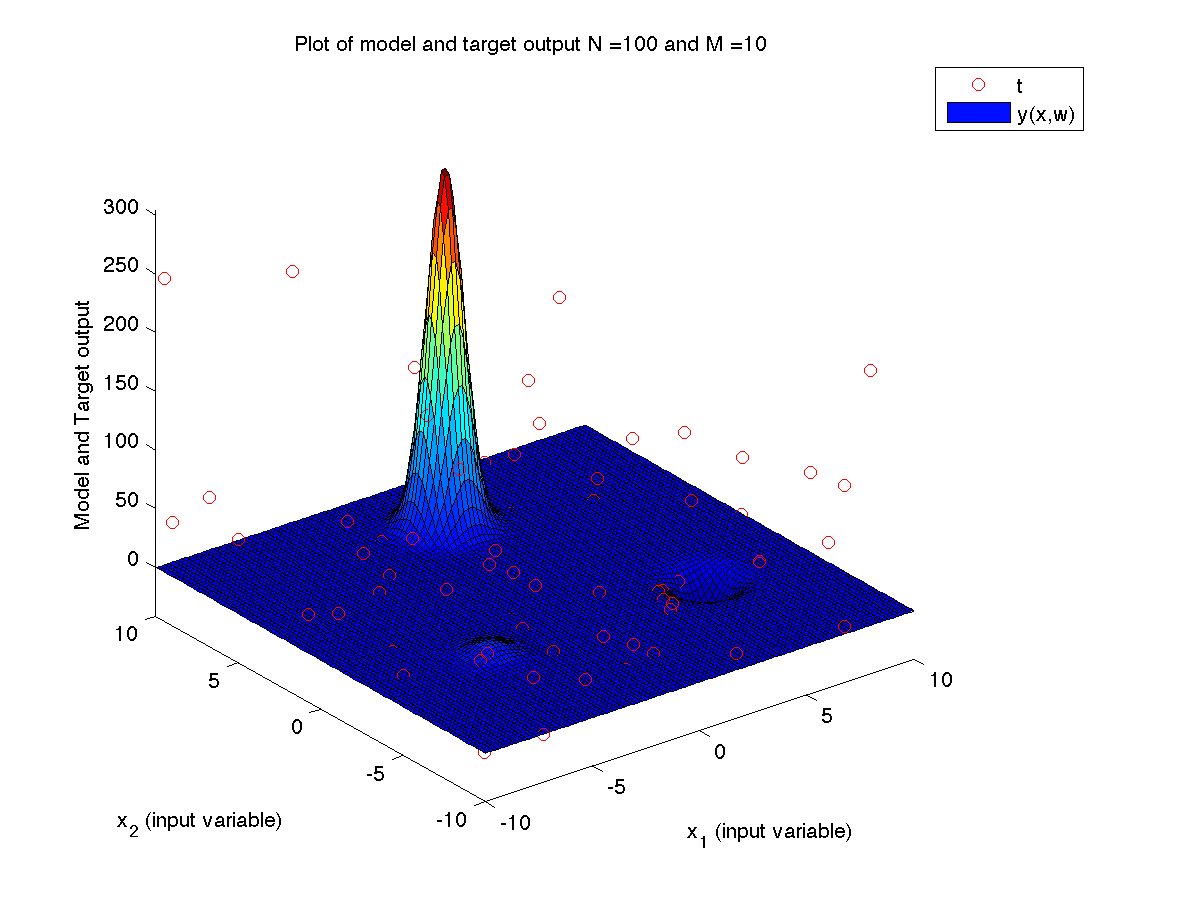
\includegraphics[width=\linewidth]{D2/VaryingM_N100M10}
\caption{N = 100 M = 10}
\end{subfigure}
\begin{subfigure}{.5\textwidth}
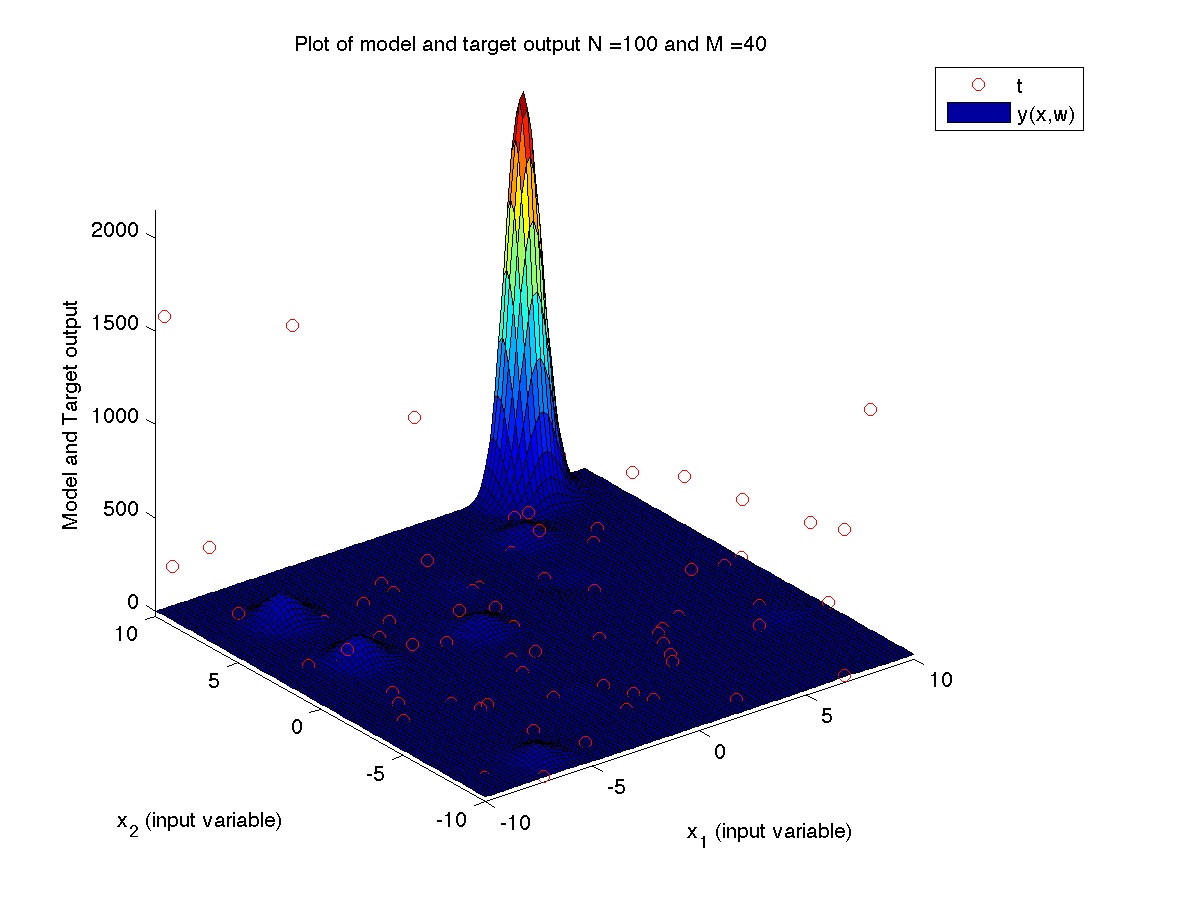
\includegraphics[width=\linewidth]{D2/VaryingM_N100M40}
\caption{N = 100 M = 40}
\end{subfigure}


\begin{subfigure}{.5\textwidth}
\centering
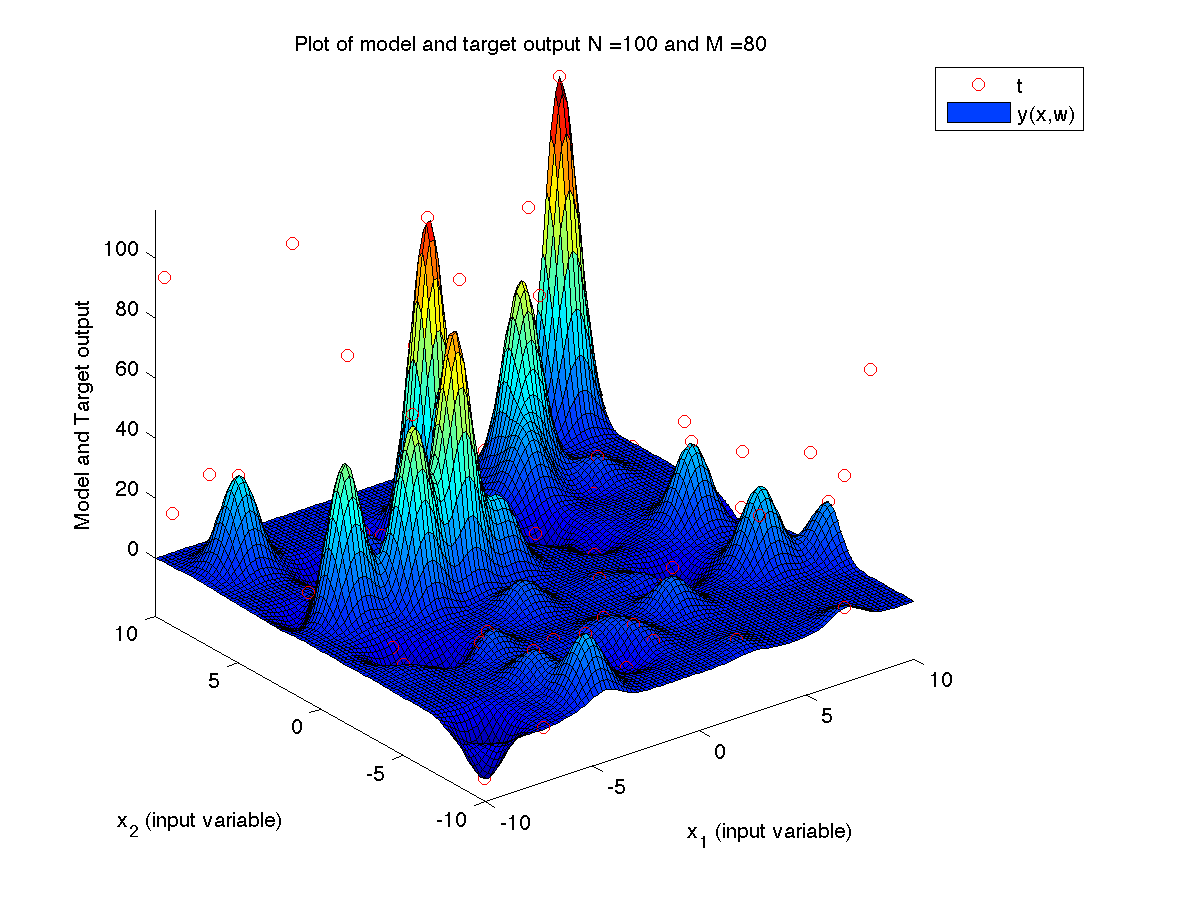
\includegraphics[width=\linewidth]{D2/VaryingM_N100M80}
\caption{N = 100 M = 80}
\end{subfigure}
\begin{subfigure}{.5\textwidth}
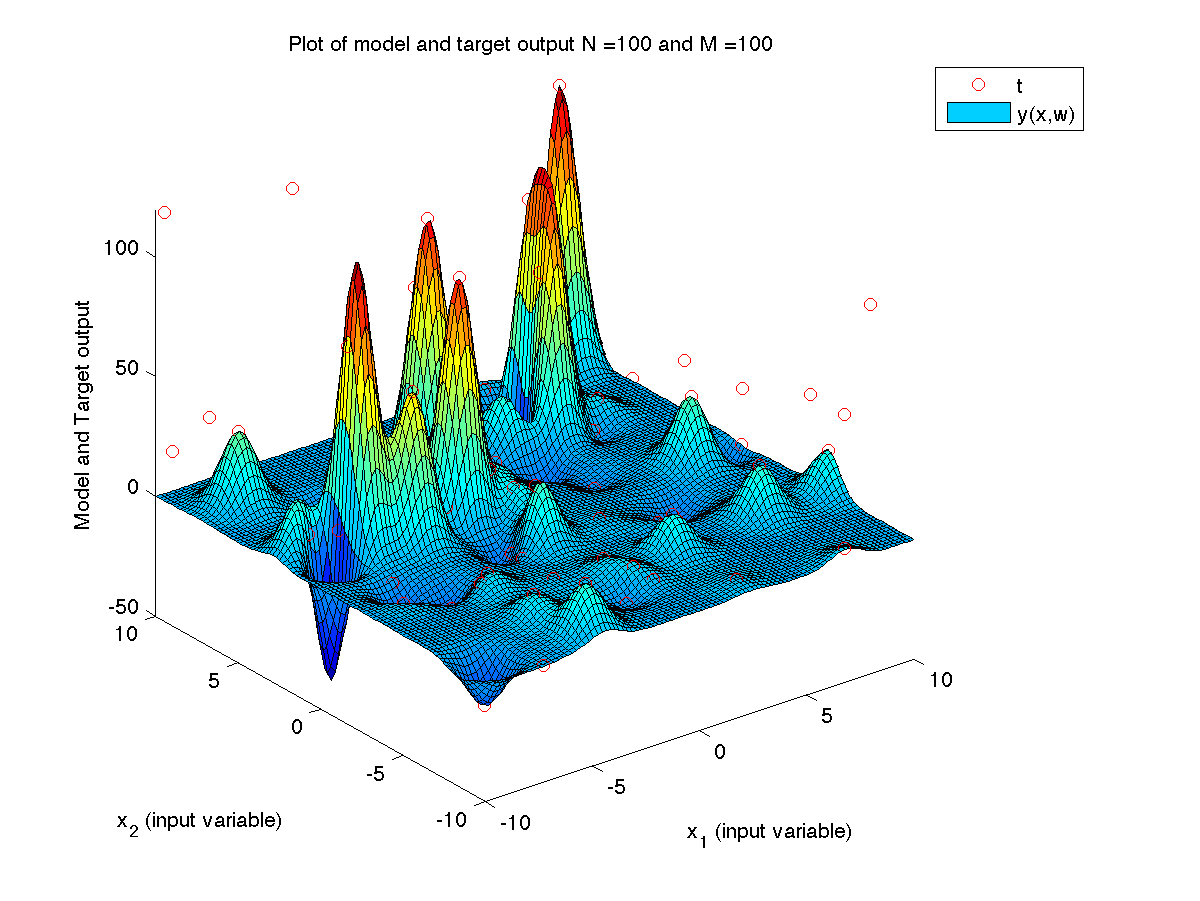
\includegraphics[width=\linewidth]{D2/VaryingM_N100M100}
\caption{N = 100 M = 100}
\end{subfigure}


\end{figure}

\textbf{Observations : \newline}
\begin{itemize}
\item TODO
\end{itemize}


\begin{flushleft}
The next set of surface plots show the variation surface fit on using training datasets of different sizes. Each of these plots are shown for a model complexity of $M = 100$. The training set size is varied as - 100,200,400,700 and 1000. The plot $N =100$ is excluded below, as it has been shown earlier.

\end{flushleft}
\begin{figure}[H]

\begin{subfigure}{.5\textwidth}
\centering
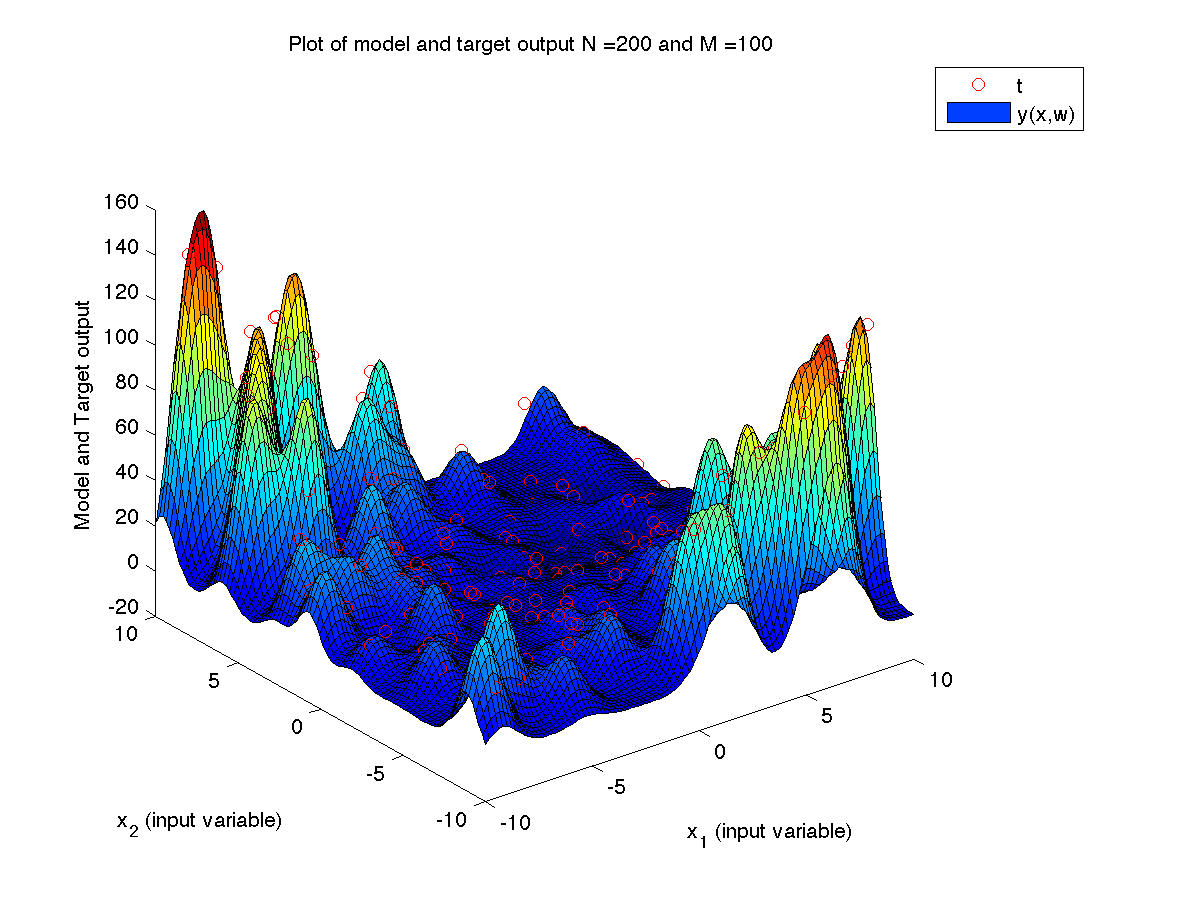
\includegraphics[width=\linewidth]{D2/VaryingN_N200M100}
\caption{N = 200 M = 100}
\end{subfigure}
\begin{subfigure}{.5\textwidth}
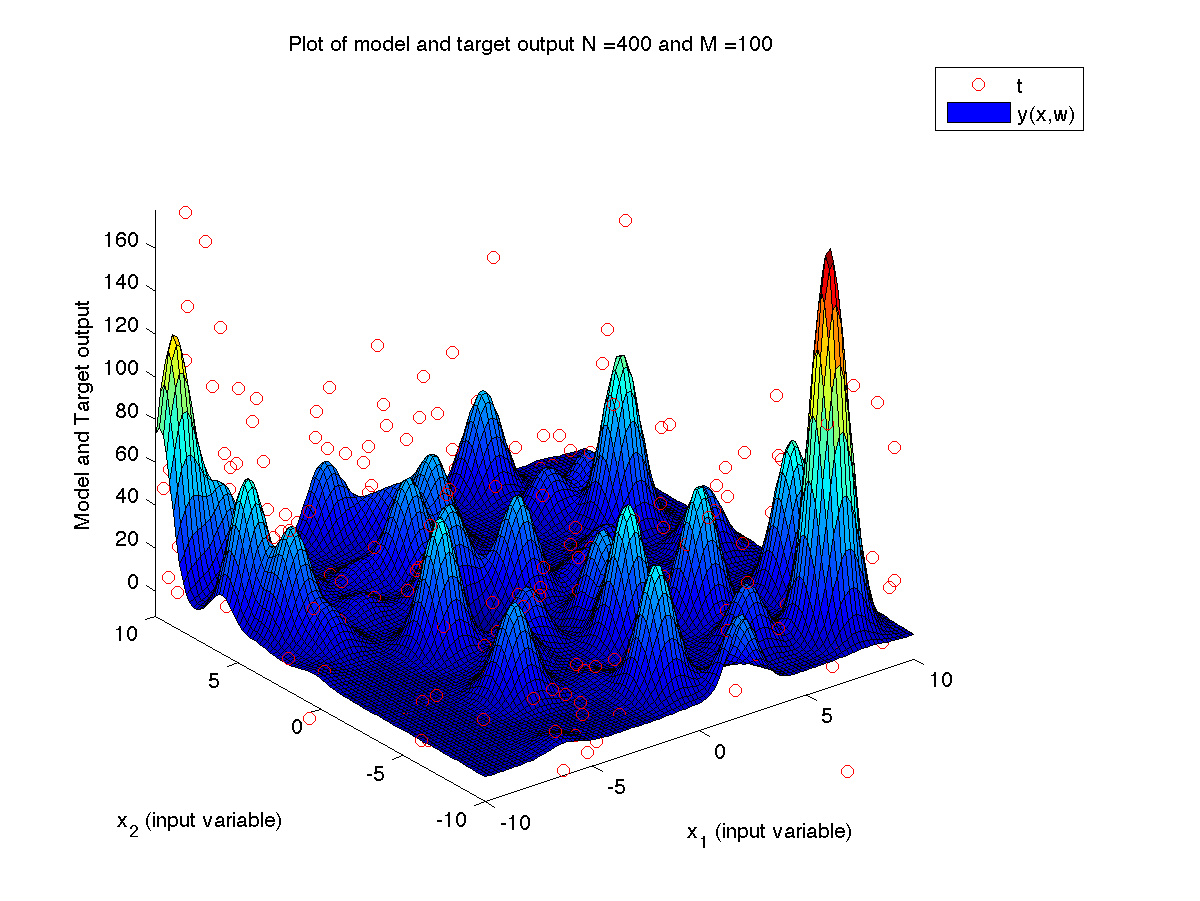
\includegraphics[width=\linewidth]{D2/VaryingN_N400M100}
\caption{N = 400 M = 100}
\end{subfigure}


\begin{subfigure}{.5\textwidth}
\centering
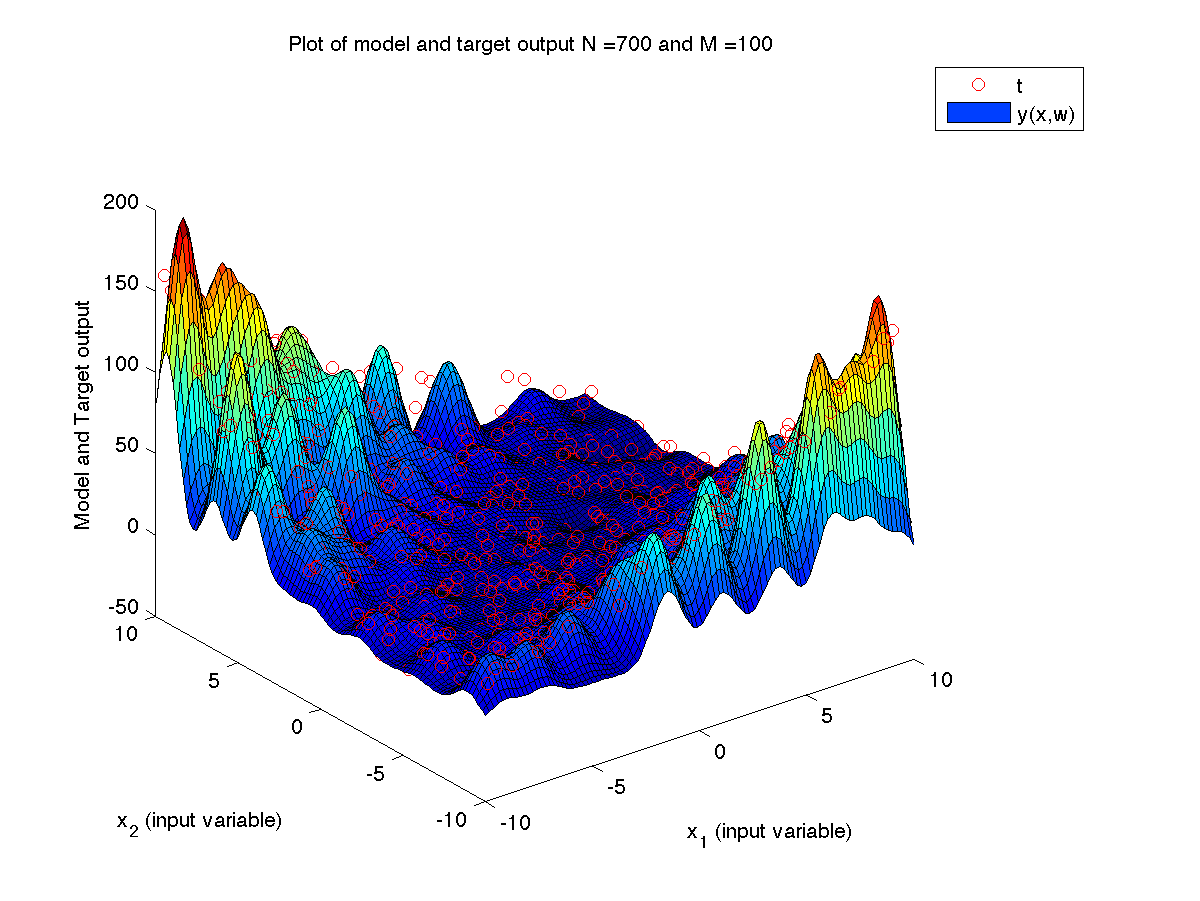
\includegraphics[width=\linewidth]{D2/VaryingN_N700M100}
\caption{N = 700 M = 100}
\end{subfigure}
\begin{subfigure}{.5\textwidth}
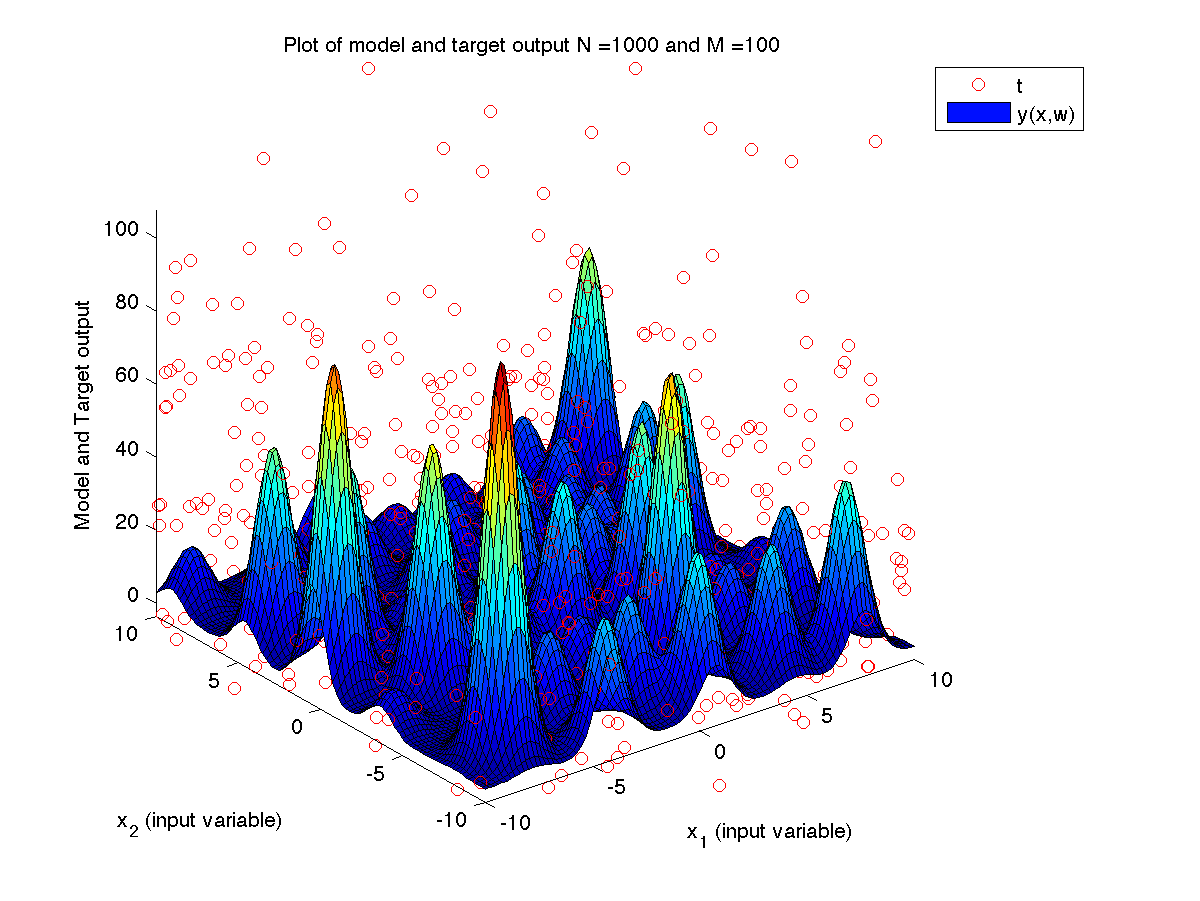
\includegraphics[width=\linewidth]{D2/VaryingN_N1000M100}
\caption{N = 1000 M = 100}
\end{subfigure}



\end{figure}


\textbf{Observations :}

\begin{itemize}
\item TODO
\end{itemize}

\begin{flushleft}
Next, we look at the effect of the regularization parameter $\lambda$ on the surface fits obtained. The plots shown below are for $N = 100$ and $M = 100$. The reason we choose $M$ to be high, is to demonstrate the effect of overfitting.

\end{flushleft}

\begin{figure}[H]

\begin{subfigure}{.5\textwidth}
\centering
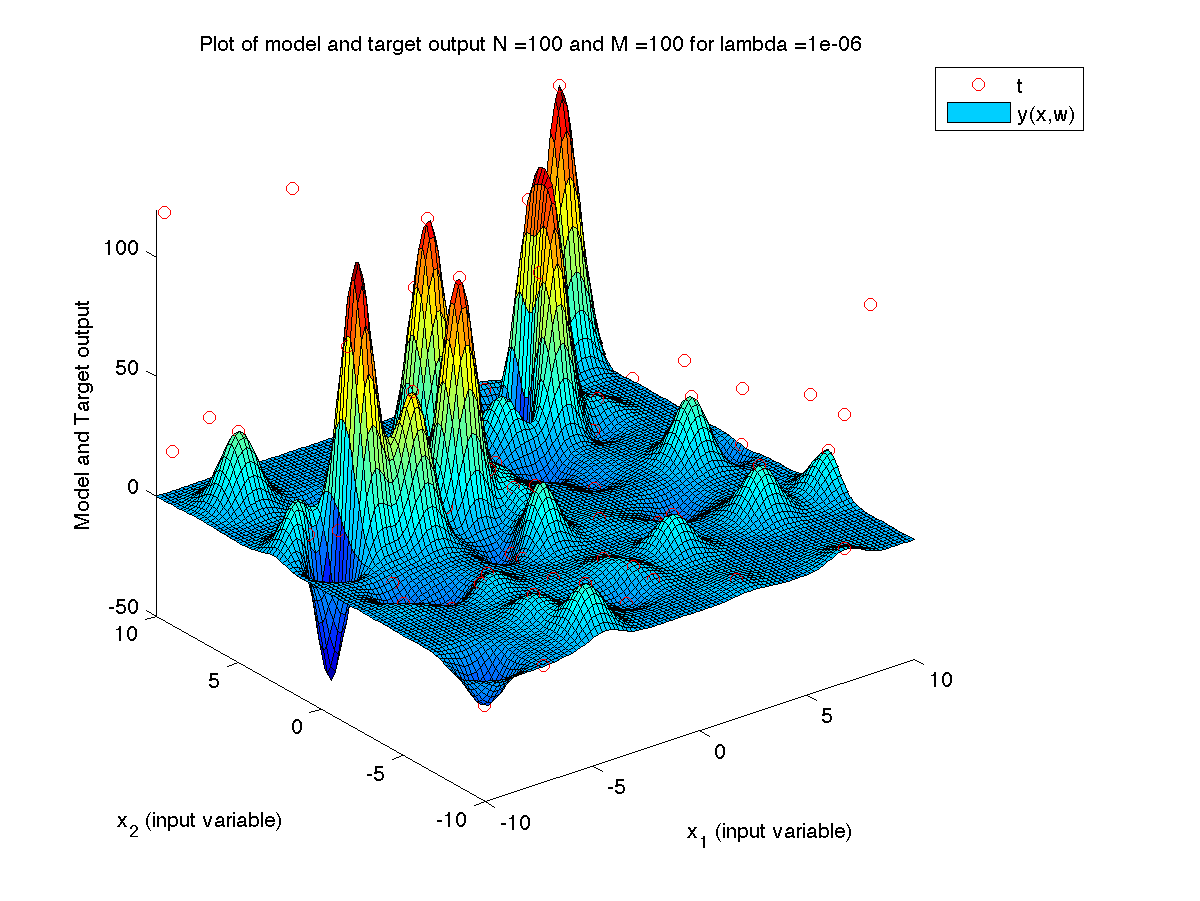
\includegraphics[width=\linewidth]{D2/Varyinglambda_N100M100lambda1e-06}
\caption{$\lambda$ = $10^{-6}$}
\end{subfigure}
\begin{subfigure}{.5\textwidth}
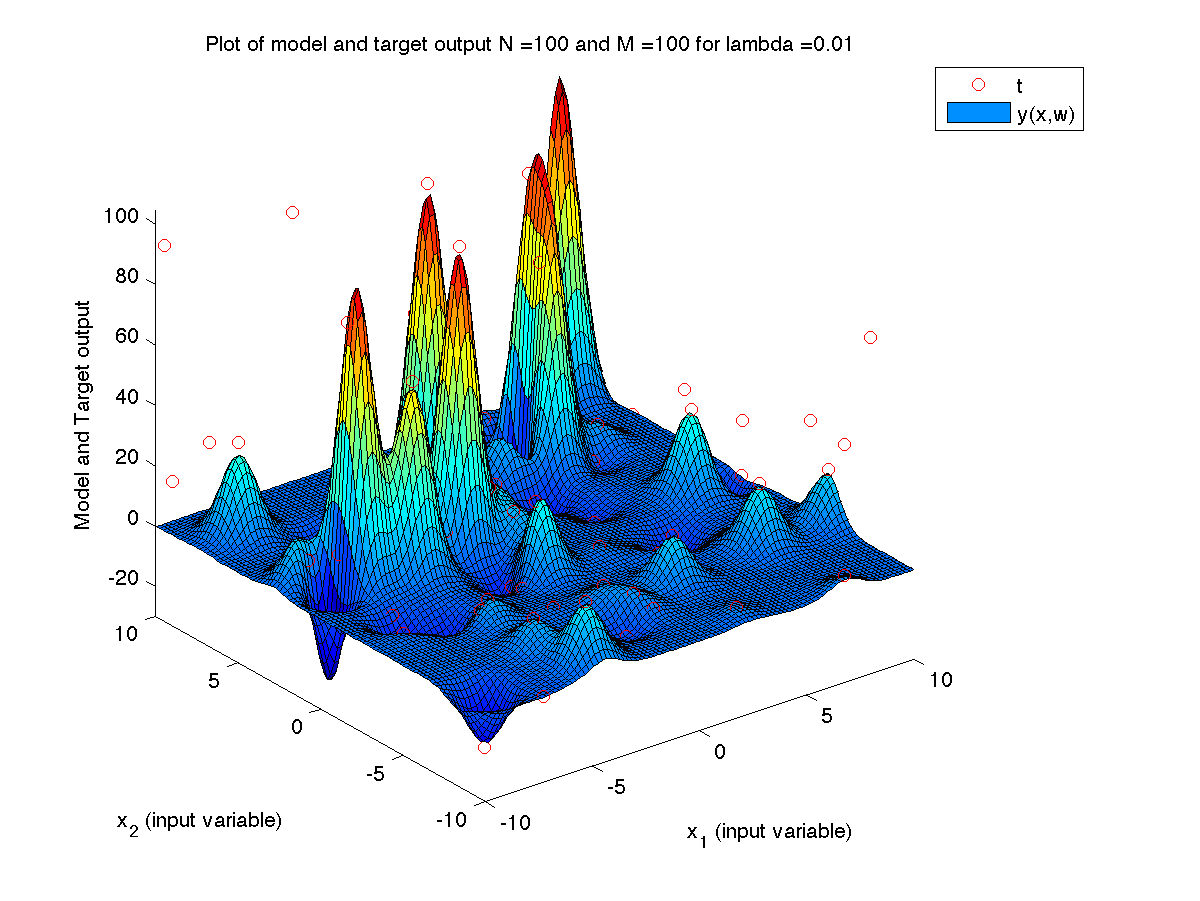
\includegraphics[width=\linewidth]{D2/Varyinglambda_N100M100lambda0_01}
\caption{$\lambda$ = 0.01}
\end{subfigure}


\begin{subfigure}{.5\textwidth}
\centering
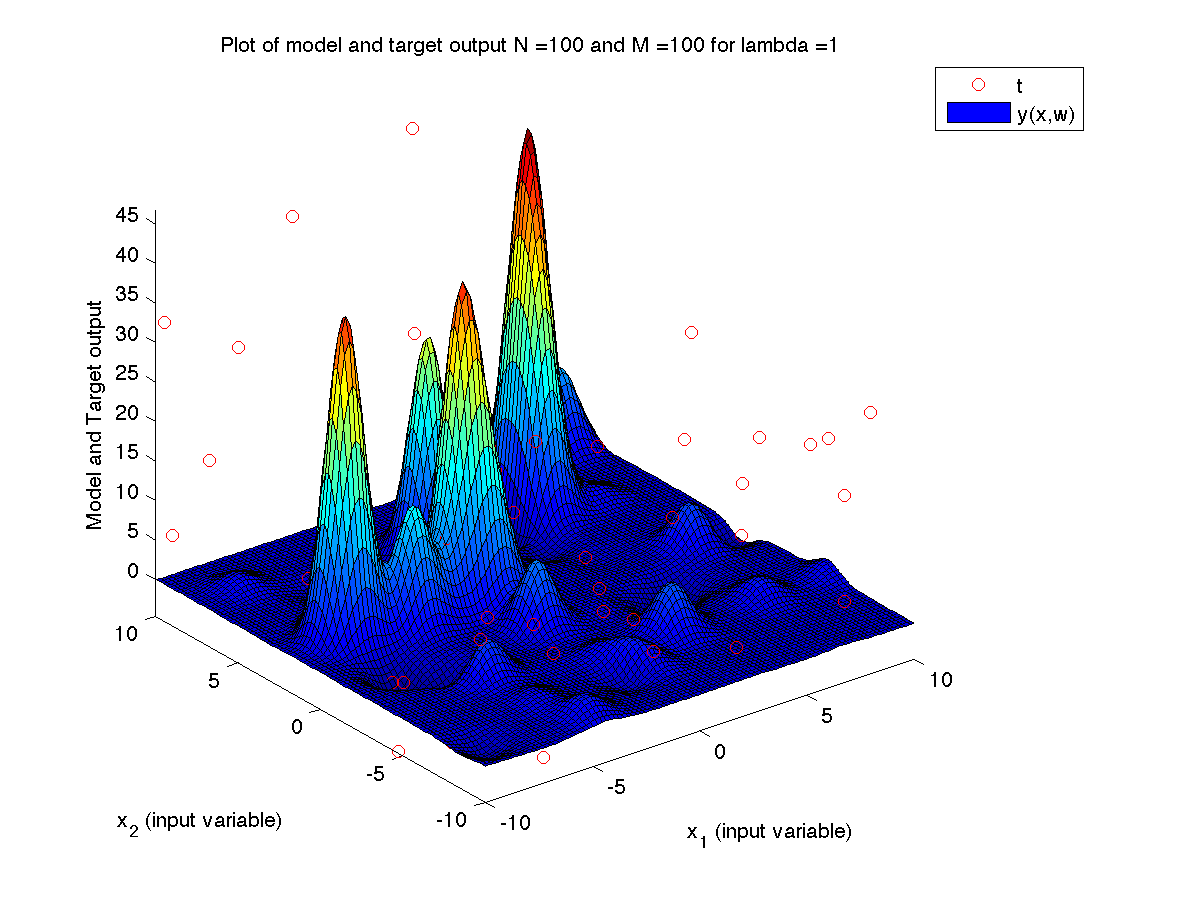
\includegraphics[width=\linewidth]{D2/Varyinglambda_N100M100lambda1}
\caption{$\lambda$ = 1}
\end{subfigure}
\begin{subfigure}{.5\textwidth}
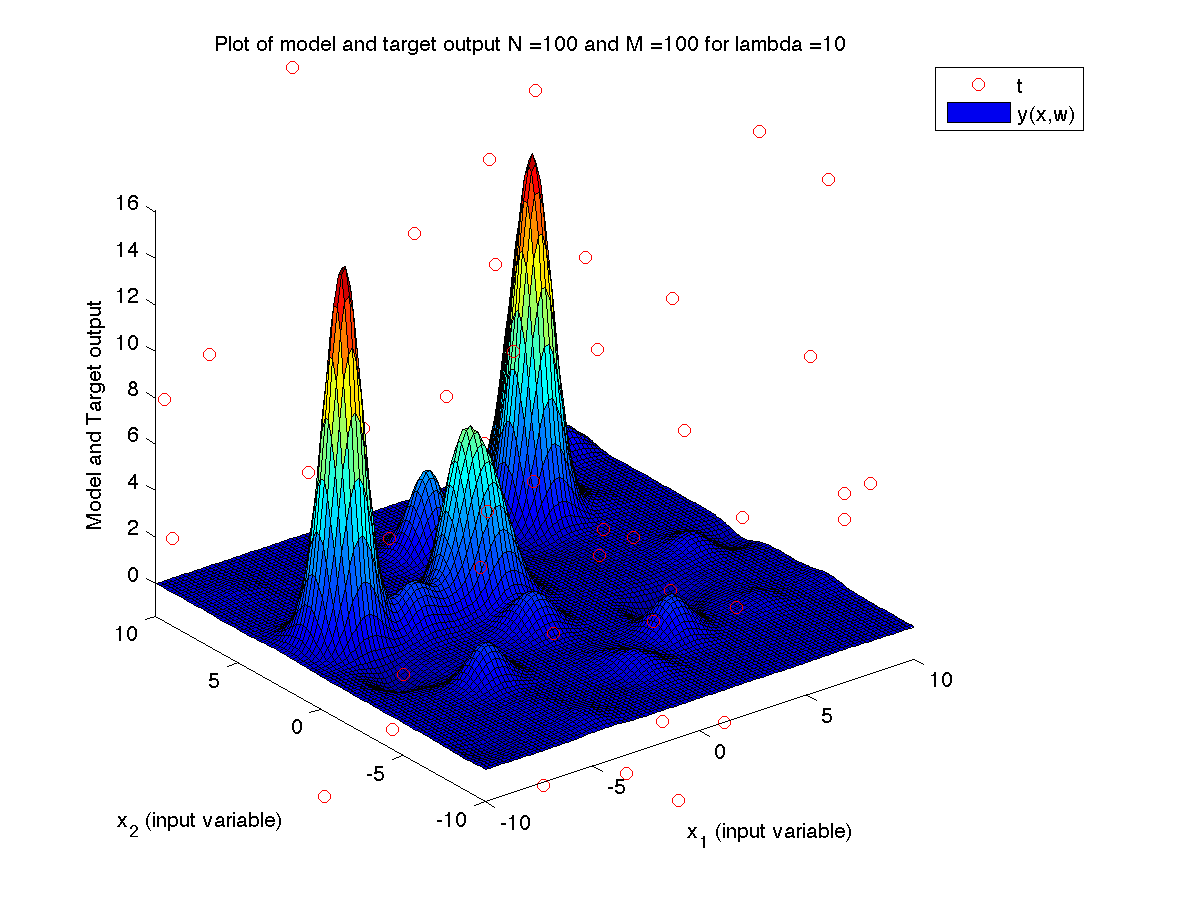
\includegraphics[width=\linewidth]{D2/Varyinglambda_N100M100lambda10}
\caption{$\lambda$ = $10$}
\end{subfigure}



\end{figure}


\textbf{Observations :}

\begin{itemize}
\item TODO
\end{itemize}


\subsection{Plots of RMS Error - Question 3}

In this section , we show the variation of RMS error, w.r.t model complexity $M$. The plots shown below are for datasets of size 100 and 1000.
Again, as earlier, for each set of plots generated on varying 1 parameter (say $M$) , the optimal value of the other parameter (say $\lambda$) is obtained by cross-validation. 
The errors have been shown on all 3 datasets for each case (test, train and validation). 

\begin{figure}[H]

\begin{subfigure}{.5\textwidth}
\centering
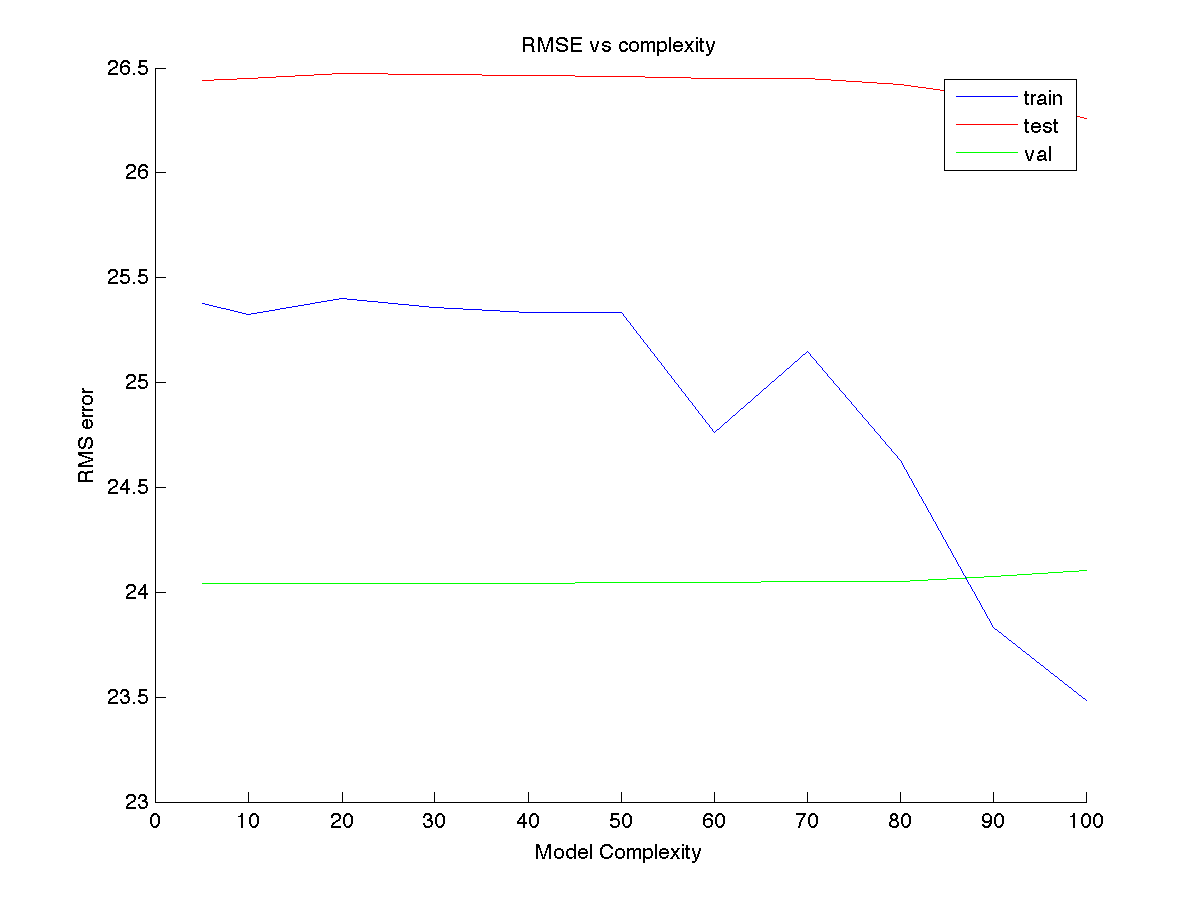
\includegraphics[width=\linewidth]{D2/RMS_complexity_100}
\caption{Varying M, Optimal $\lambda$, 100 train size}
\end{subfigure}
\begin{subfigure}{.5\textwidth}
%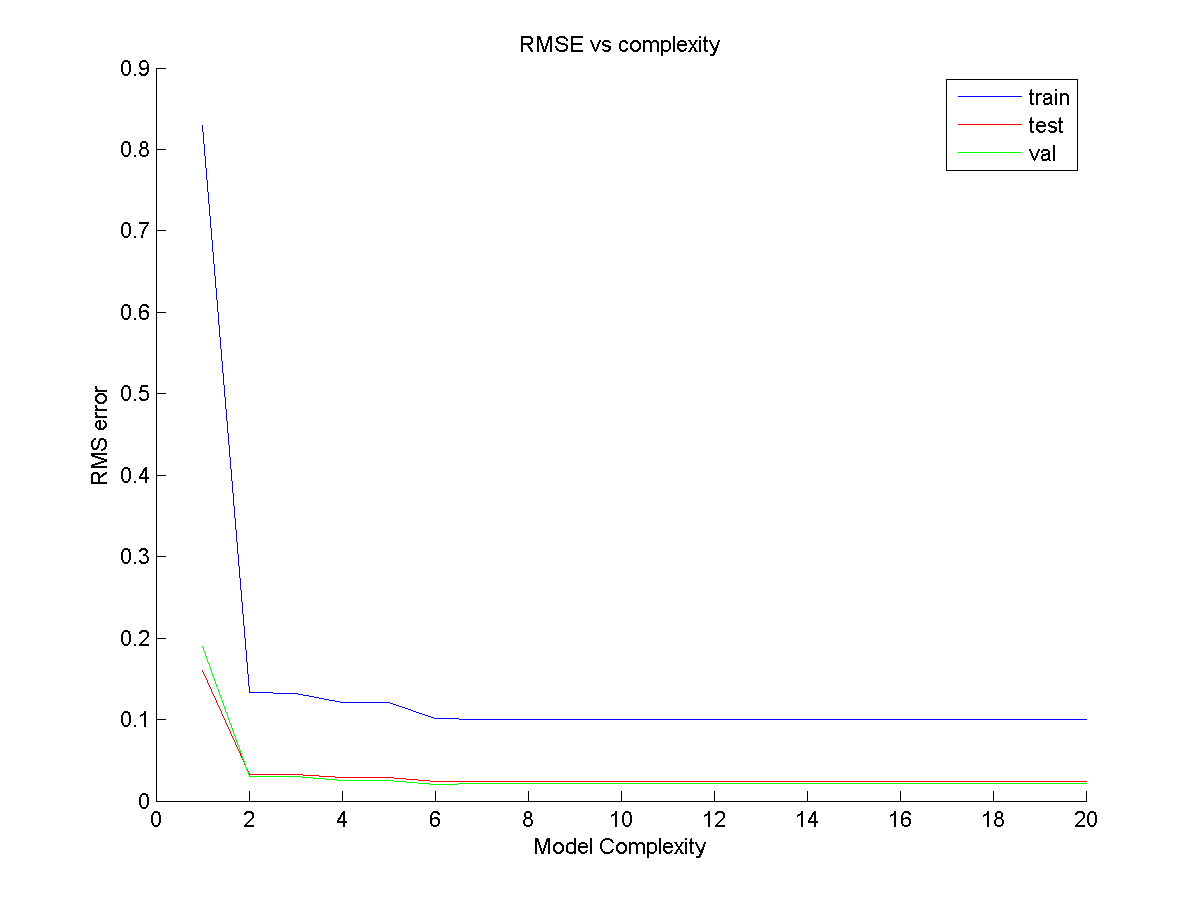
\includegraphics[width=\linewidth]{D2/RMS_complexity_1000}
\caption{Varying M, Optimal $\lambda$, ? train size}
\end{subfigure}


\begin{subfigure}{.5\textwidth}
\centering
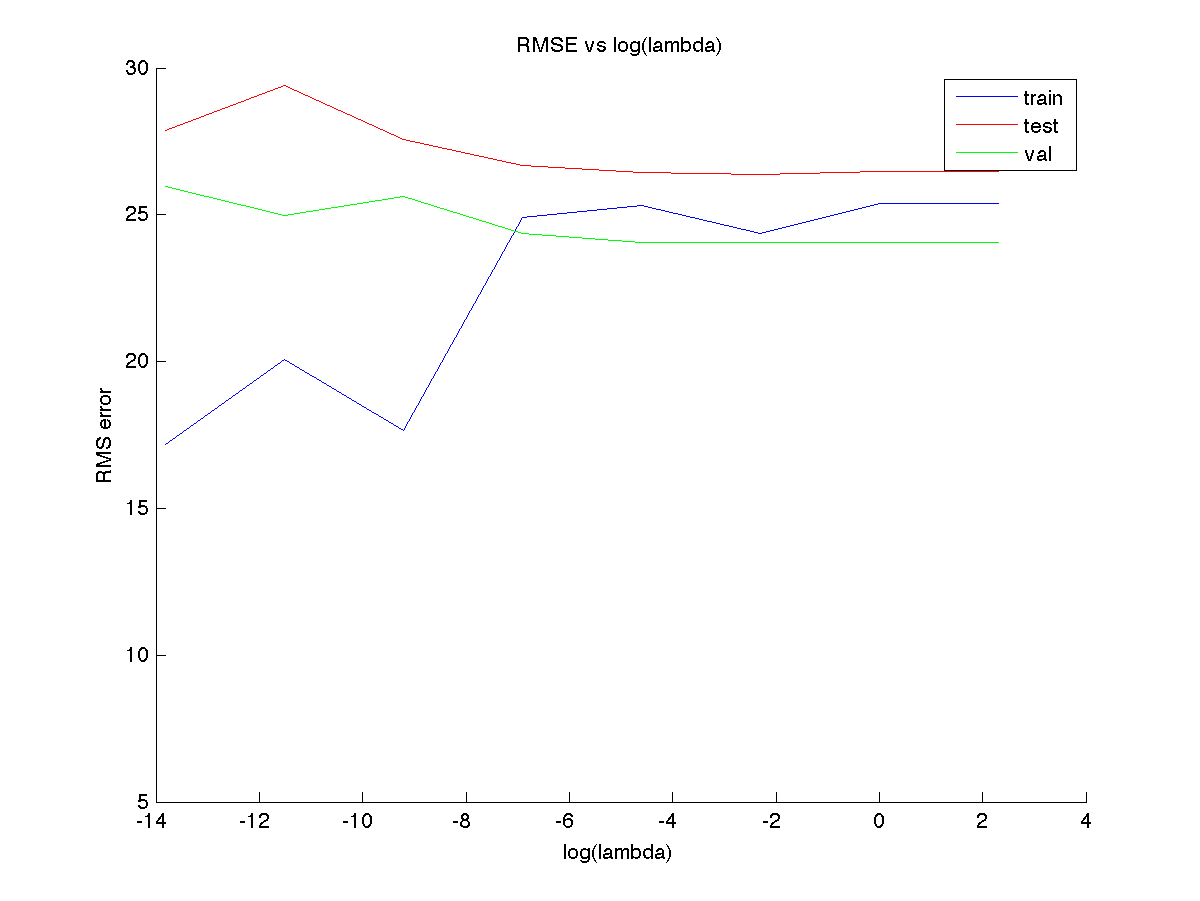
\includegraphics[width=\linewidth]{D2/RMS_lambda_100}
\caption{Optimal M, Varying $\lambda$, 100 train size}
\end{subfigure}
\begin{subfigure}{.5\textwidth}
%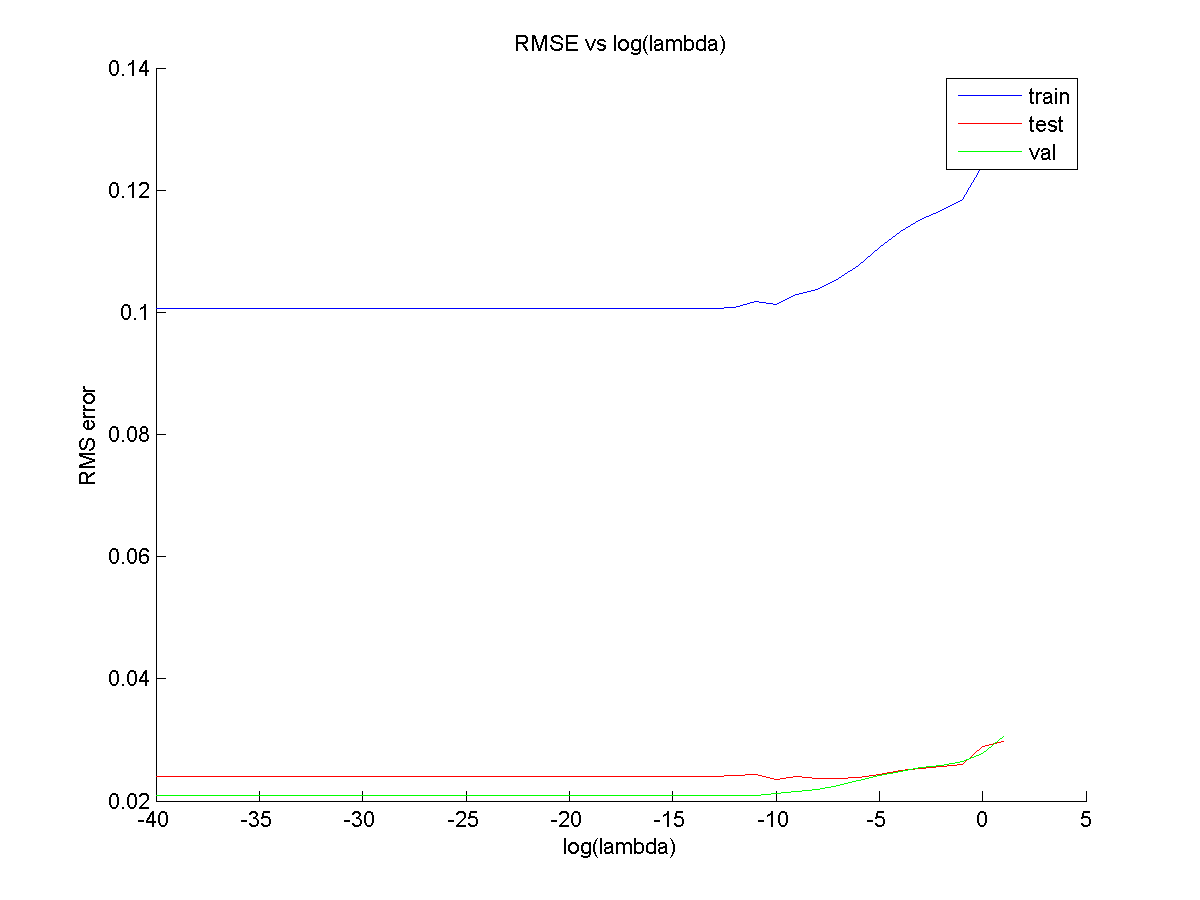
\includegraphics[width=\linewidth]{D2/RMS_lambda_1000}
\caption{Optimal M, Varying $\lambda$, ? train size}
\end{subfigure}


\textbf{Observations :}

\begin{itemize}
\item TODO
\end{itemize}


\end{figure}



\subsection{Scatter plots of target and model output - Question 4}

TODO - add some text here varying M etc.

\begin{figure}[H]

\begin{subfigure}{.5\textwidth}
\centering
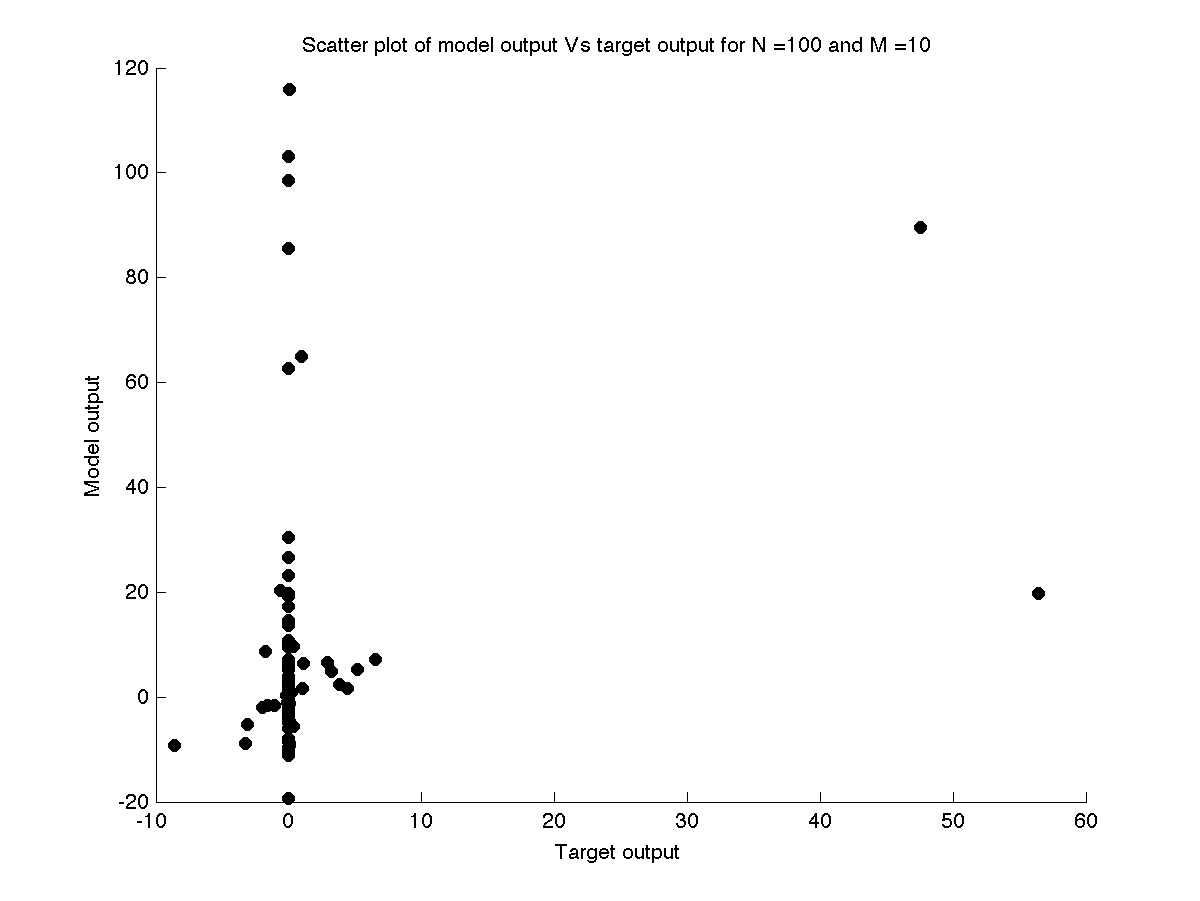
\includegraphics[width=\linewidth]{D2/Scatter/VaryingM_N100M10}
\caption{N = 100 M = 10}
\end{subfigure}
\begin{subfigure}{.5\textwidth}
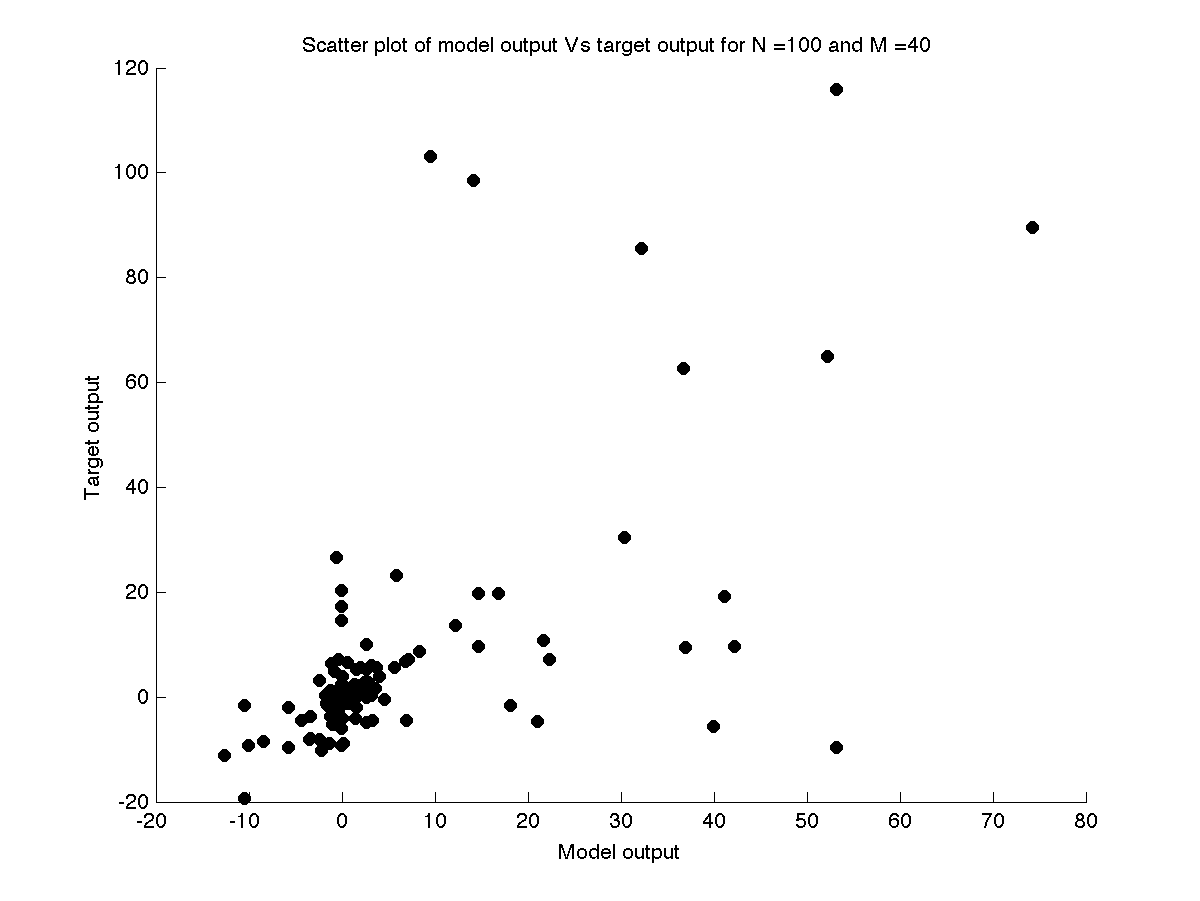
\includegraphics[width=\linewidth]{D2/Scatter/VaryingM_N100M40}
\caption{N = 100 M = 40}
\end{subfigure}


\begin{subfigure}{.5\textwidth}
\centering
\includegraphics[width=\linewidth]{D2/Scatter/VaryingM_N100M80}
\caption{N = 100 M = 80}
\end{subfigure}
\begin{subfigure}{.5\textwidth}
\includegraphics[width=\linewidth]{D2/Scatter/VaryingM_N100M100}
\caption{N = 100 M = 100}
\end{subfigure}


\end{figure}

\textbf{Observations : \newline}
\begin{itemize}
\item TODO
\end{itemize}



TODO - Add some text here - varying N etc.
\begin{figure}[H]

\begin{subfigure}{.5\textwidth}
\centering
\includegraphics[width=\linewidth]{D2/Scatter/VaryingN_N200M100}
\caption{N = 200 M = 100}
\end{subfigure}
\begin{subfigure}{.5\textwidth}
\includegraphics[width=\linewidth]{D2/Scatter/VaryingN_N400M100}
\caption{N = 400 M = 100}
\end{subfigure}


\begin{subfigure}{.5\textwidth}
\centering
\includegraphics[width=\linewidth]{D2/Scatter/VaryingN_N700M100}
\caption{N = 700 M = 100}
\end{subfigure}
\begin{subfigure}{.5\textwidth}
\includegraphics[width=\linewidth]{D2/Scatter/VaryingN_N1000M100}
\caption{N = 1000 M = 100}
\end{subfigure}



\end{figure}


\textbf{Observations :}

\begin{itemize}
\item TODO
\end{itemize}


TODO - Add some text here - varying lambda etc.

\begin{figure}[H]

\begin{subfigure}{.5\textwidth}
\centering
\includegraphics[width=\linewidth]{D2/Scatter/Varyinglambda_N100M100lambda1e-06}
\caption{$\lambda$ = $10^{-6}$}
\end{subfigure}
\begin{subfigure}{.5\textwidth}
\includegraphics[width=\linewidth]{D2/Scatter/Varyinglambda_N100M100lambda0_01}
\caption{$\lambda$ = 0.01}
\end{subfigure}


\begin{subfigure}{.5\textwidth}
\centering
\includegraphics[width=\linewidth]{D2/Scatter/Varyinglambda_N100M100lambda1}
\caption{$\lambda$ = 1}
\end{subfigure}
\begin{subfigure}{.5\textwidth}
%\includegraphics[width=\linewidth]{D2/Scatter/Varyinglambda_N100M100lambda10}
\caption{$\lambda$ = $10$}
\end{subfigure}



\end{figure}


\textbf{Observations :}

\begin{itemize}
\item TODO
\end{itemize}



\end{document}
